\clearpage

\section{\label{result}Results and Discussion}

\subsection{\label{result:pt}$p_{\rm T}$ Spectra and Integrated Yields}

Figure~\ref{D0_spectra} shows the efficiency corrected $D^0$ invariant yield at mid-rapidity ($|y|<1$) vs. transverse momentum ($p_{\rm T}$) in 0--10\%, 10--20\%, 20--40\%, 40--60\%, 60--80\% and 0--80\% Au + Au collisions at $\sqrt{s_{_{\rm NN}}}$ = 200\,GeV. $D^0$ invariant spectra in some centrality bins are arbitrarily scaled with factors indicated on the plot for clarity. Dashed lines depict fits to these spectra with the following Levy function

\begin{equation}
\frac{d^2N}{2\pi p_{\rm T}dp_{\rm T}dy} = \frac{1}{2\pi}\frac{dN}{dy}\frac{(n-1)(n-2)}{nT(nT+m_0(n-2))}\bigg(1+\frac{\sqrt{p_{\rm T}^2+m_0^2}-m_0}{nT}\bigg)^{-n}
\end{equation}

where $m_0$ is the $D^0$ particle mass and $\frac{dN}{dy}$, $T$ and $n$ are the free parameters. The Levy function fit shows nice descriptions to the $D^0$ spectra in all centrality bins up to 8\,GeV/$c$.

\begin{figure}
\centering
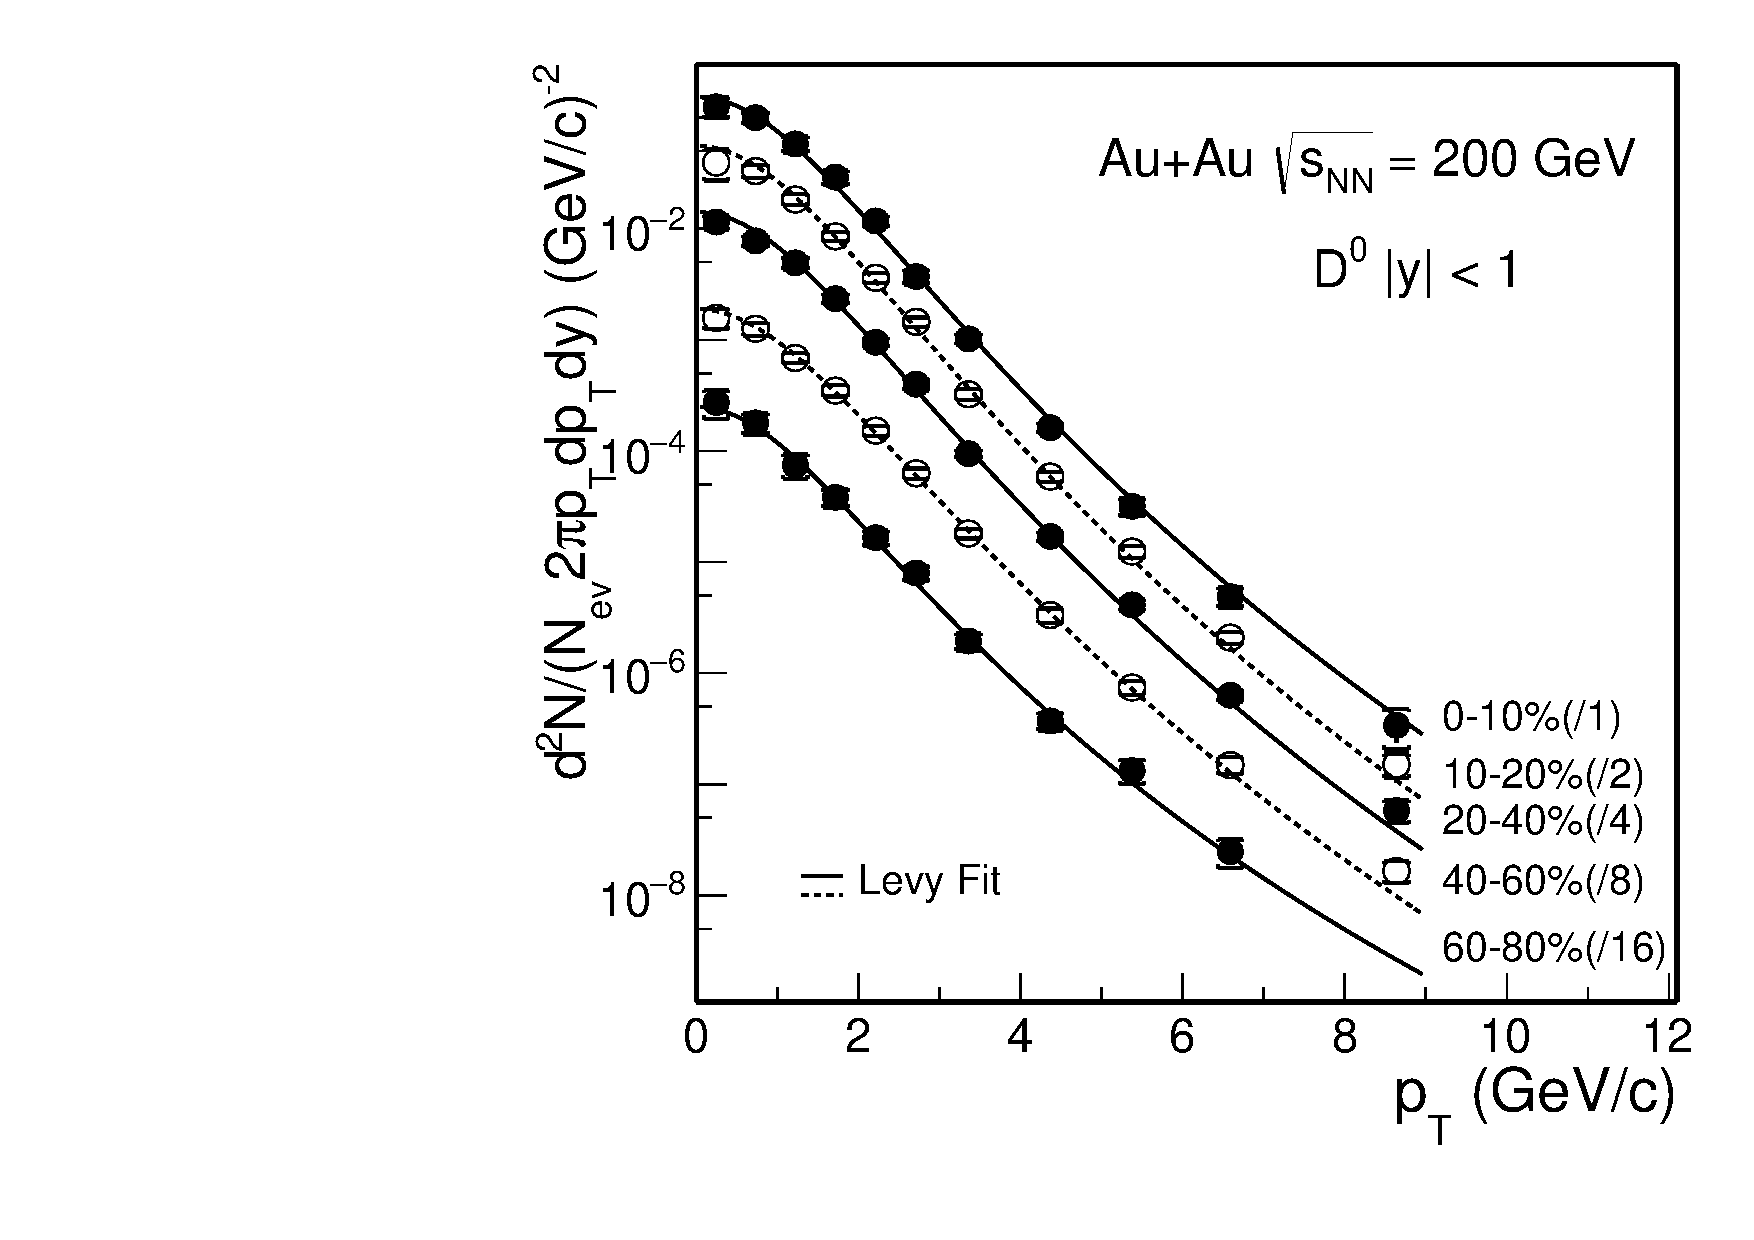
\includegraphics[width=0.68\textwidth]{figure/Run14_D0HFT/D0_spectra.pdf}
\caption{$D^{0}$ invariant yield at mid-rapidity ($|y|<1$) vs. transverse momentum for different centrality classes in Au + Au collisions at $\sqrt{s_{_{\rm NN}}}$ = 200\,GeV. Error bars (not visible for many data points) indicate statistical uncertainties and brackets depict systematical uncertainties. Global systematic uncertainties in $B.R.$ and $N_{\rm bin}$ are not plotted. Solid and dashed lines depict Levy function fits.}
\label{D0_spectra} 
\end{figure}

\begin{figure}
\centering
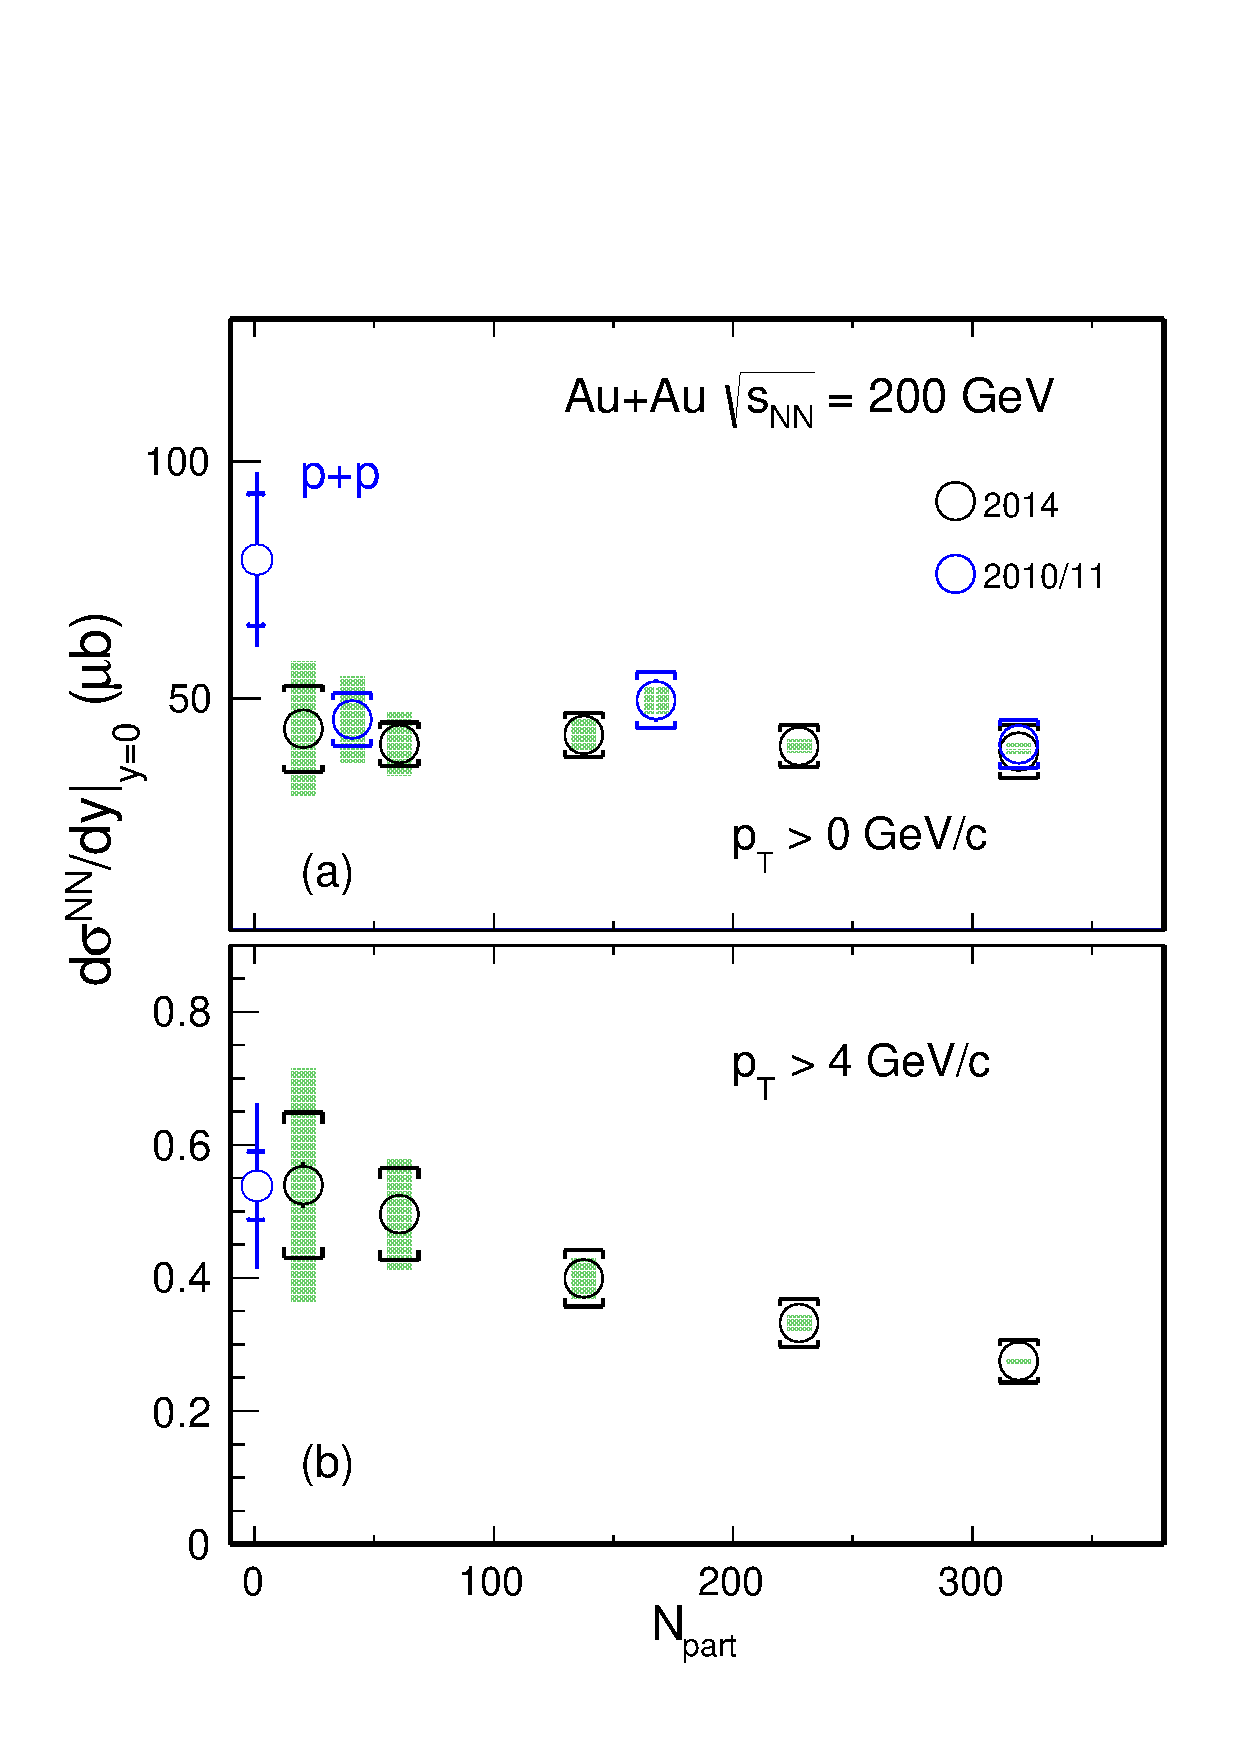
\includegraphics[width=0.68\textwidth]{figure/Run14_D0HFT/Xsection_D0.pdf}
\caption{$D^{0}$ integrated cross sections per nucleon-nucleon collision at mid-rapidity for $p_{\rm T}>0$ and $p_{\rm T}>4$\,GeV/$c$ regions as a function of centrality $N_{\rm bin}$.}
\label{Xsection_D0} 
\end{figure}

After got the efficiency corrected pt spectra, the integrated $D^0$ yield was also obtained as shown in the next equation.

\begin{equation}
  d\sigma = \sum \frac{dN_{i}}{dy}\frac{1}{Events}\frac{1}{N_{bin}} * 42e^3 * 0.0388
\end{equation}

Fig.\ref{Xsection_D0} shows the integrated cross section per nucleon-nucleon collision in different centralities.

\subsection{\label{result:collectivity}Collectivity}

\subsubsection{\label{result:collectivity:mT}$m_{\rm T}$ Spectra}

Transverse mass spectra have often used to study the collectivity of produced hadrons in heavy-ion collisions. Figure~\ref{mTFit_D0} shows the $D^{0}$ invariant yield at mid-rapidity ($|y|<1$) vs. transverse kinetic energy ($m_{\rm T}$ - $m_{0}$) for different centrality classes in Au + Au collisions at $\sqrt{s_{_{\rm NN}}}$ = 200\,GeV, where $m_{\rm T} = \sqrt{p_{\rm T}^2+m_0^2}$ and $m_0$ is the $D^0$ meson mass. Solid and dashed black lines depict exponential function fits to various centrality bins up to $m_{\rm T} = 3m_{0}$ and the fit function is shown below

\begin{equation}
\frac{d^2N}{2\pi m_{\rm T}dm_{\rm T}dy} = \frac{dN/dy}{2\pi T_{\rm eff}(m_0+T_{\rm eff})}e^{-(m_{\rm T}-m_0)/T_{\rm eff}}
\end{equation}

A power-law function (shown below) is also used to fit the spectrum in 60--80\% centrality bin. 

\begin{equation}
\frac{d^2N}{2\pi p_{\rm T}dp_{\rm T}dy} = \frac{dN}{dy}\frac{4(n-1)(n-2)}{2\pi (n-3)^2\langle p_{\rm T} \rangle ^2}\bigg(1+\frac{2p_{\rm T}}{\langle p_{\rm T} \rangle (n-3)}\bigg)^{-n}
\end{equation}

where $dN/dy$, $\langle p_{\rm T}\rangle$, and $n$ are three free parameters. 

The power-law function fit shows a better description to the 60--80\% centrality data indicating the $D^0$ meson production in this peripheral bin is close to the perturbative QCD feature. The $D^0$ meson spectra in more central collisions can be well described by the expotential function fit suggesting the $D^0$ mesons have gained collectivity in the medium evolution in these collisions.

\begin{figure}
\centering
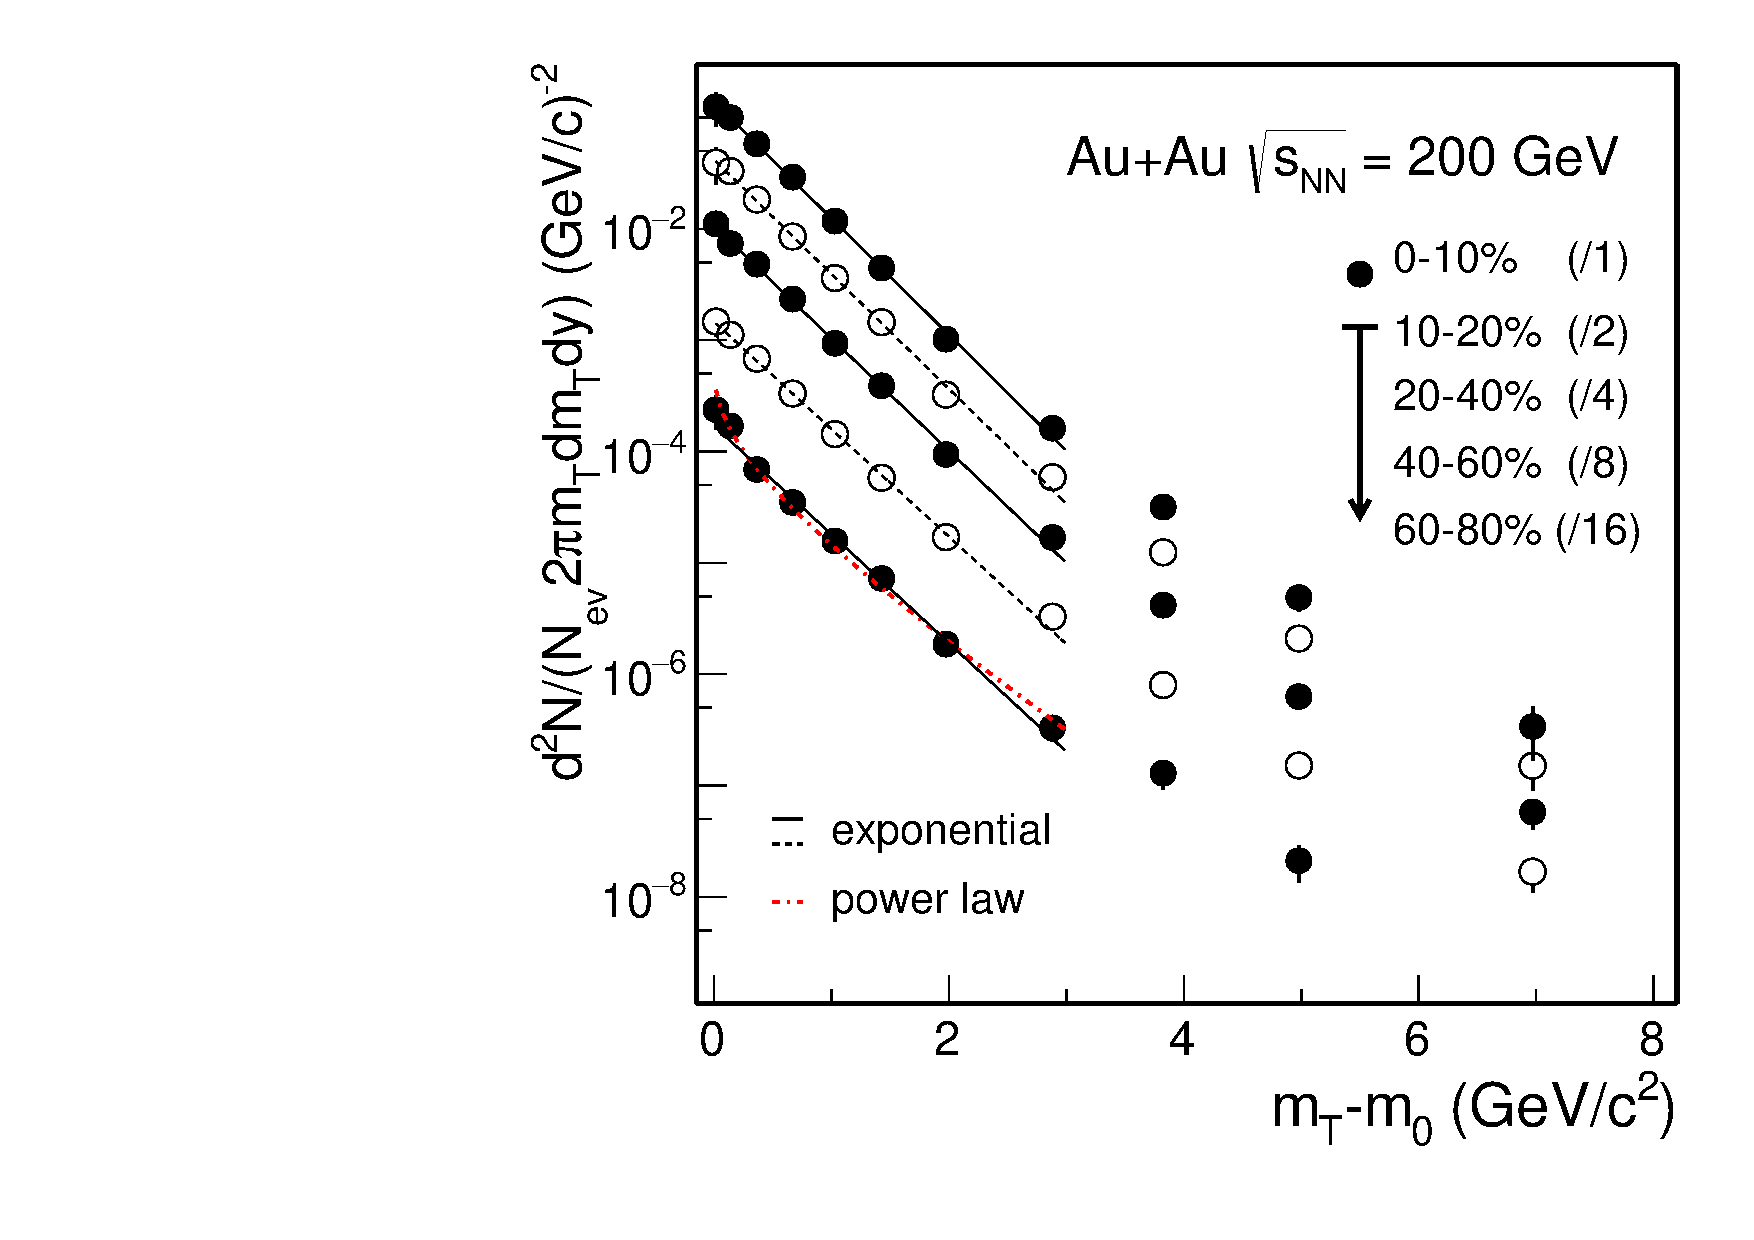
\includegraphics[width=0.68\textwidth]{figure/Run14_D0HFT/mTFit_D0.pdf}
\caption{$D^{0}$ invariant yield at mid-rapidity ($|y|<1$) vs. transverse kinetic energy ($m_{T}$ - $m_{0}$) for different centrality classes in Au + Au collisions at $\sqrt{s_{_{\rm NN}}}$ = 200\,GeV. Error bars (not visible for many data points) indicate statistical uncertainties and brackets depict systematical uncertainties. Global systematic uncertainties in $B.R.$ and $N_{\rm bin}$ are not plotted. Solid and dashed black lines depict exponential function fits and the dot-dashe line depict a power-law function fit to the spectrum in 60--80\% centrality bin.}
\label{mTFit_D0} 
\end{figure}

Figure~\ref{Teff_D0} shows the $m_{\rm T}$ spectra slope parameter $T_{\rm eff}$ (obtained from the expontential fit described above) vs. collision centrality. Statistical and point-to-point systematic uncertainties, but no global systematic uncertainties, are added quadratically when performing the expontial fit. Therefore uncertainties shown in this plot are the total uncertainties on this fit parameter. The obtained $T_{\rm eff}$ parameter increases from peripheral to central collisions, suggesting more collectivity that $D^0$ mesons gain in more central collisions. 

\begin{figure}
\centering
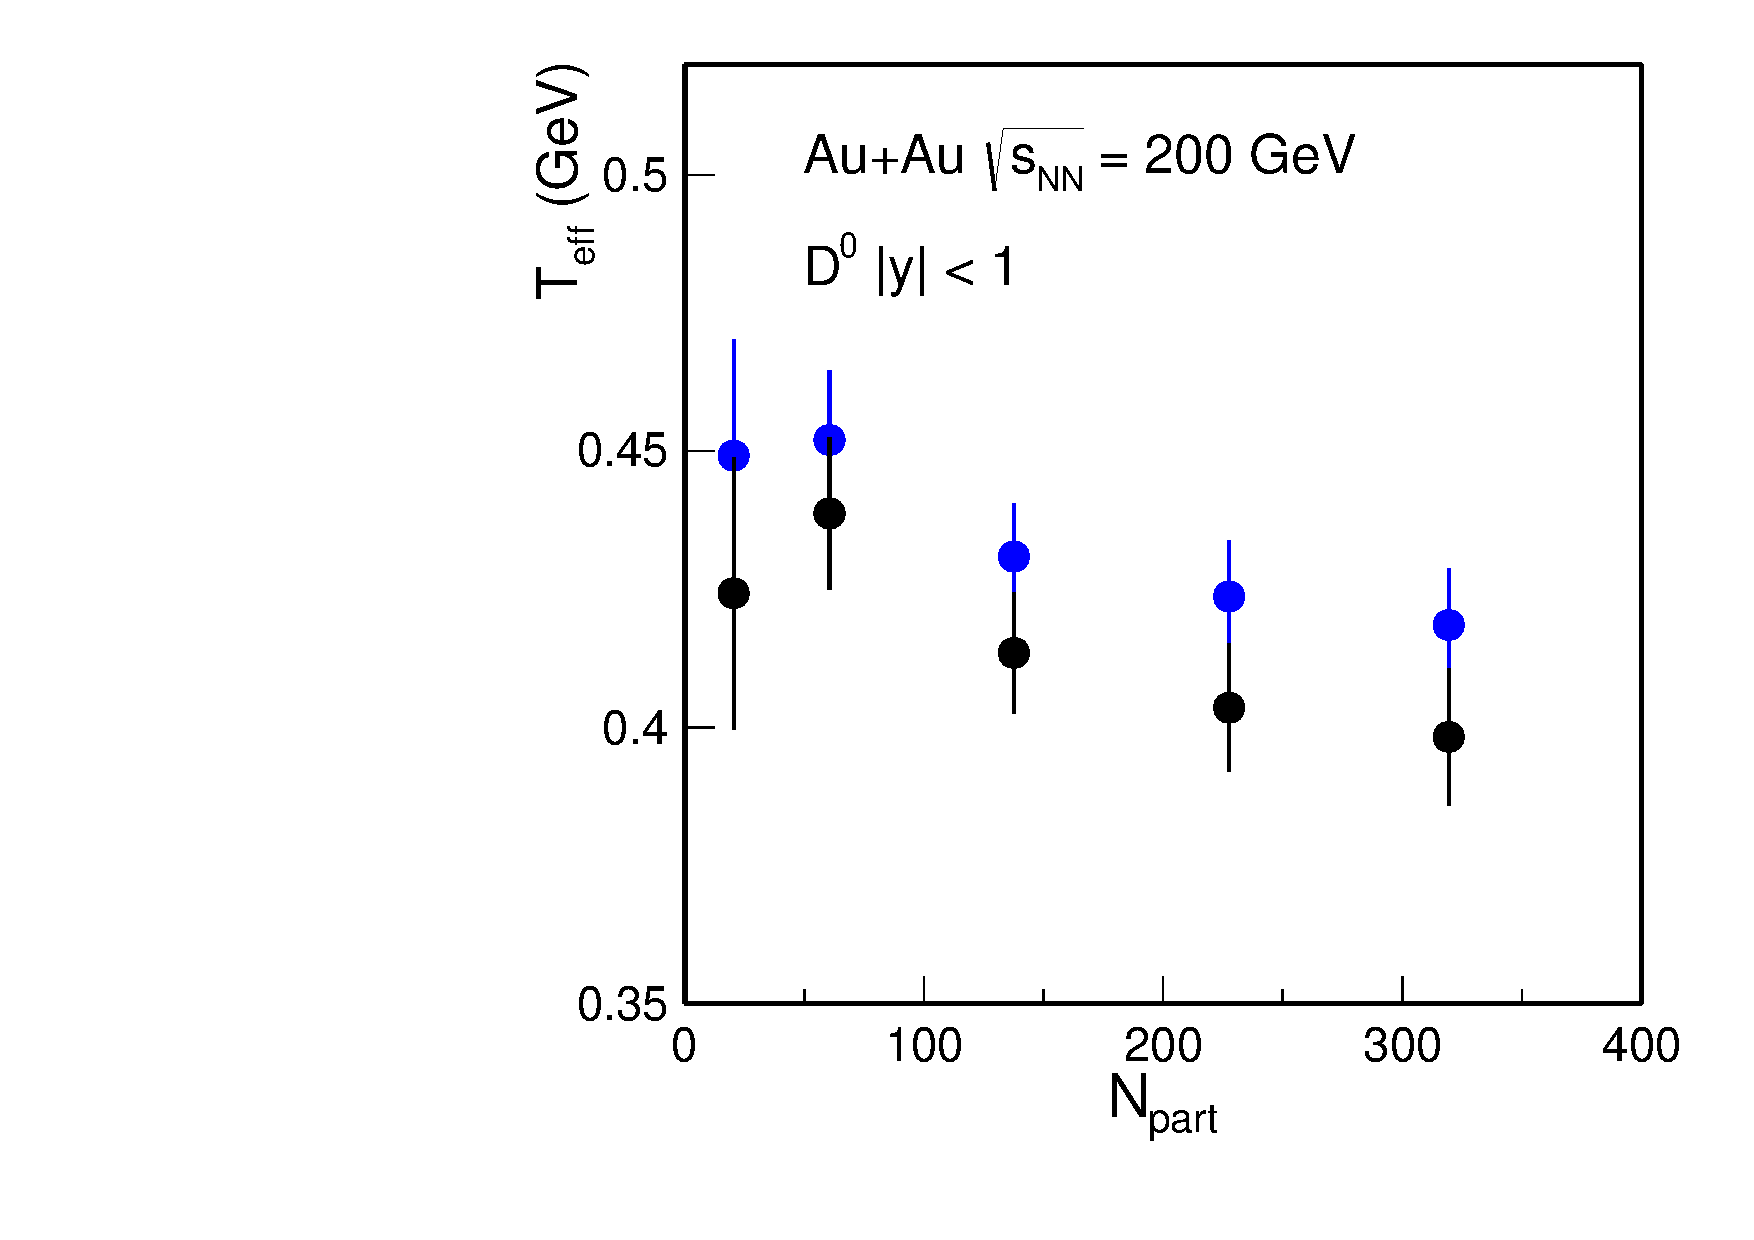
\includegraphics[width=0.68\textwidth]{figure/Run14_D0HFT/Teff_D0.pdf}
\caption{$T_{eff}$ vs. $N_{bin}$ for different centrality classes in Au + Au collisions at $\sqrt{s_{_{\rm NN}}}$ = 200\,GeV.}
\label{Teff_D0} 
\end{figure}

The obtained slope parameter $T_{\rm eff}$ for $D^0$ mesons is compared to other light and strange hadrons measured at RHIC. %Figure~\ref{figure:mTFit_ALL} shows the exponential function fit to various hadron spectra 
Figure~\ref{Teff_ALL} summarizes the slope parameter $T_{\rm eff}$ for various identified hadrons ($\pi^{\pm}$,$K^{\pm}$,$p$/$\bar{p}$,$\phi$,$\Lambda$,$\Xi^-$,$\Omega$,$D^0$ and $J/\psi$) in central Au + Au collisions at $\sqrt{s_{_{\rm NN}}}$ = 200\,GeV. All fits are performed up to $m_{\rm T} = 3m_{0}$.


\begin{figure}
\centering
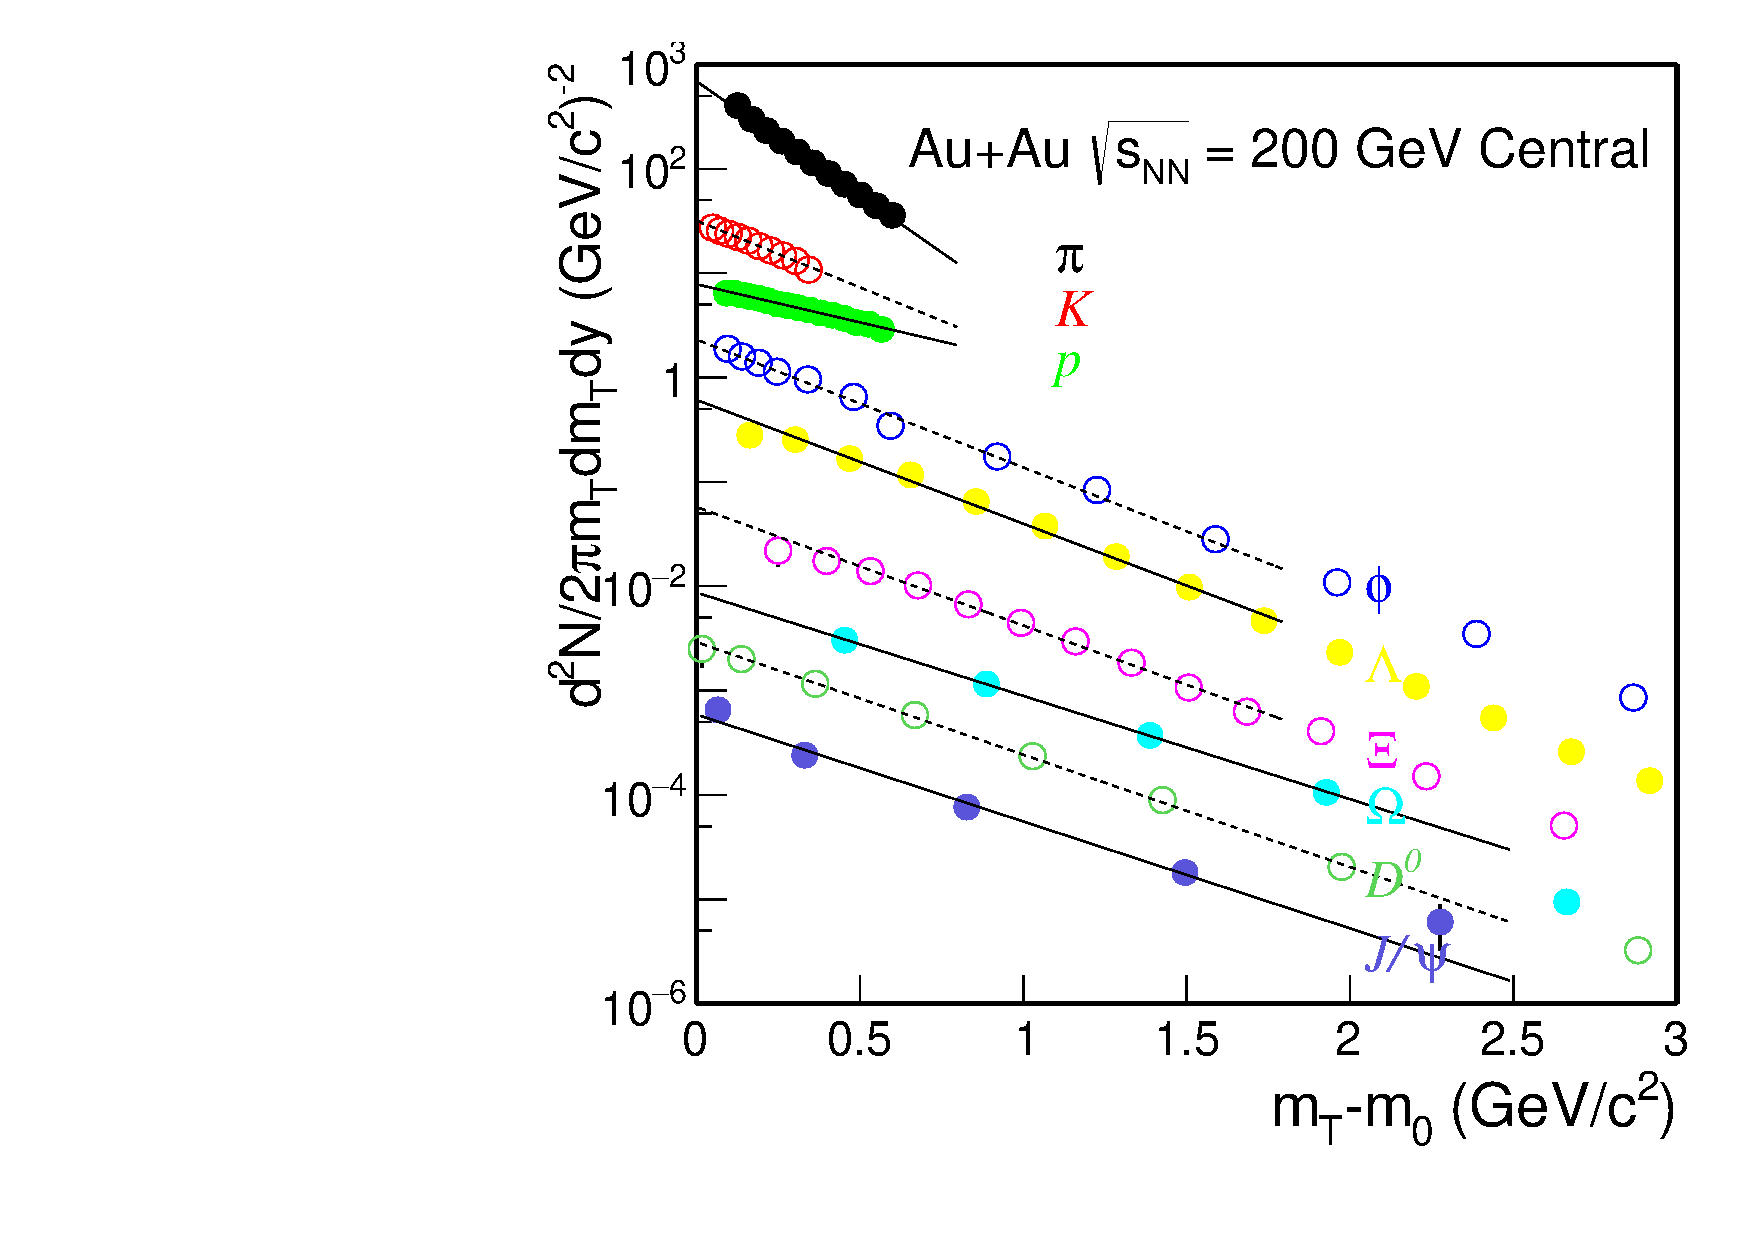
\includegraphics[width=0.68\textwidth]{figure/Run14_D0HFT/mTFit_ALL.pdf}
\caption{$D^{0}$ invariant yield at mid-rapidity ($|y|<1$) vs. ($m_{T}$ - $m_{0}$) for central collisions in Au + Au collisions at $\sqrt{s_{_{\rm NN}}}$ = 200\,GeV.}
\label{mTFit_ALL} 
\end{figure}

\begin{figure}
\centering
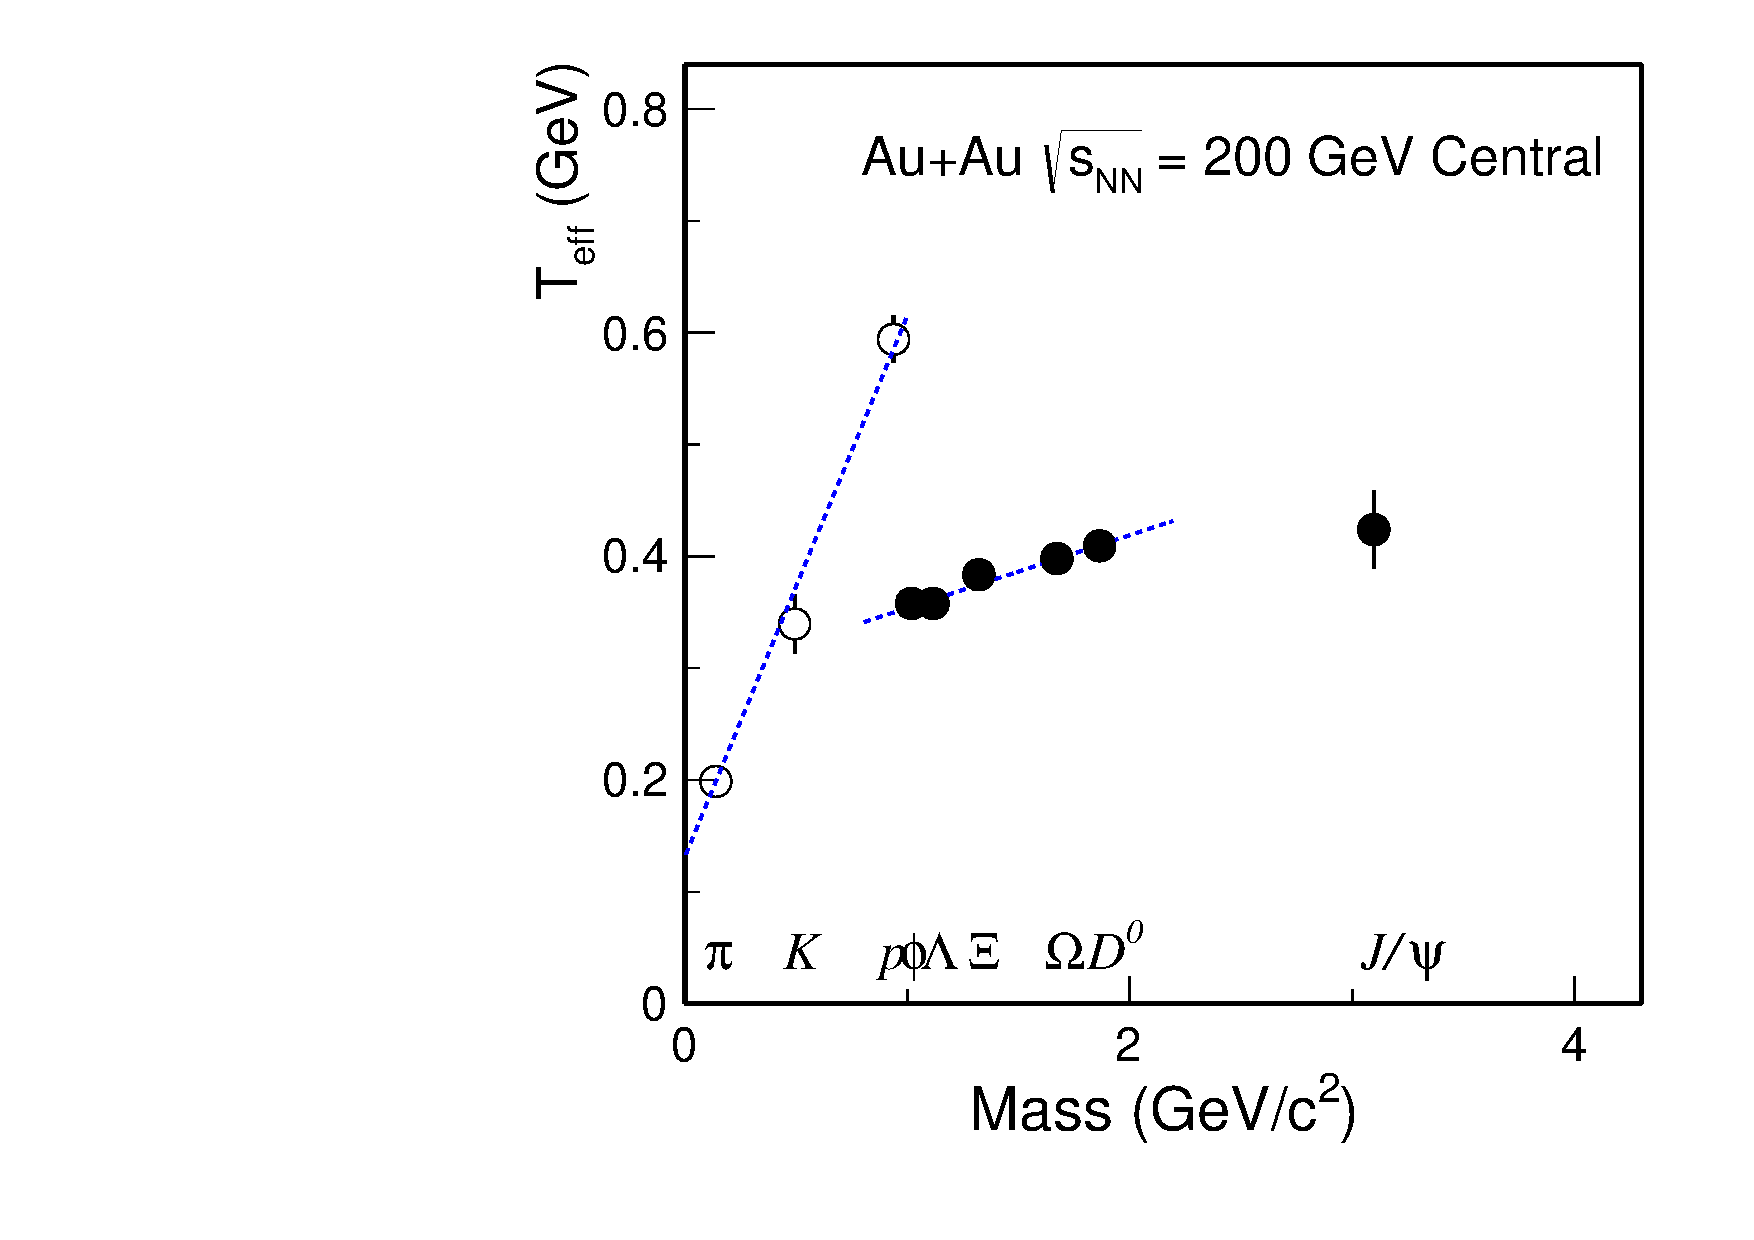
\includegraphics[width=0.68\textwidth]{figure/Run14_D0HFT/Teff_ALL.pdf}
\caption{$T_{\rm eff}$ for different particles in central Au + Au collisions at $\sqrt{s_{_{\rm NN}}}$ = 200\,GeV.}
\label{Teff_ALL} 
\end{figure}


\subsubsection{\label{result:collectivity:BW}Blast-wave fit}

\begin{figure}
\centering
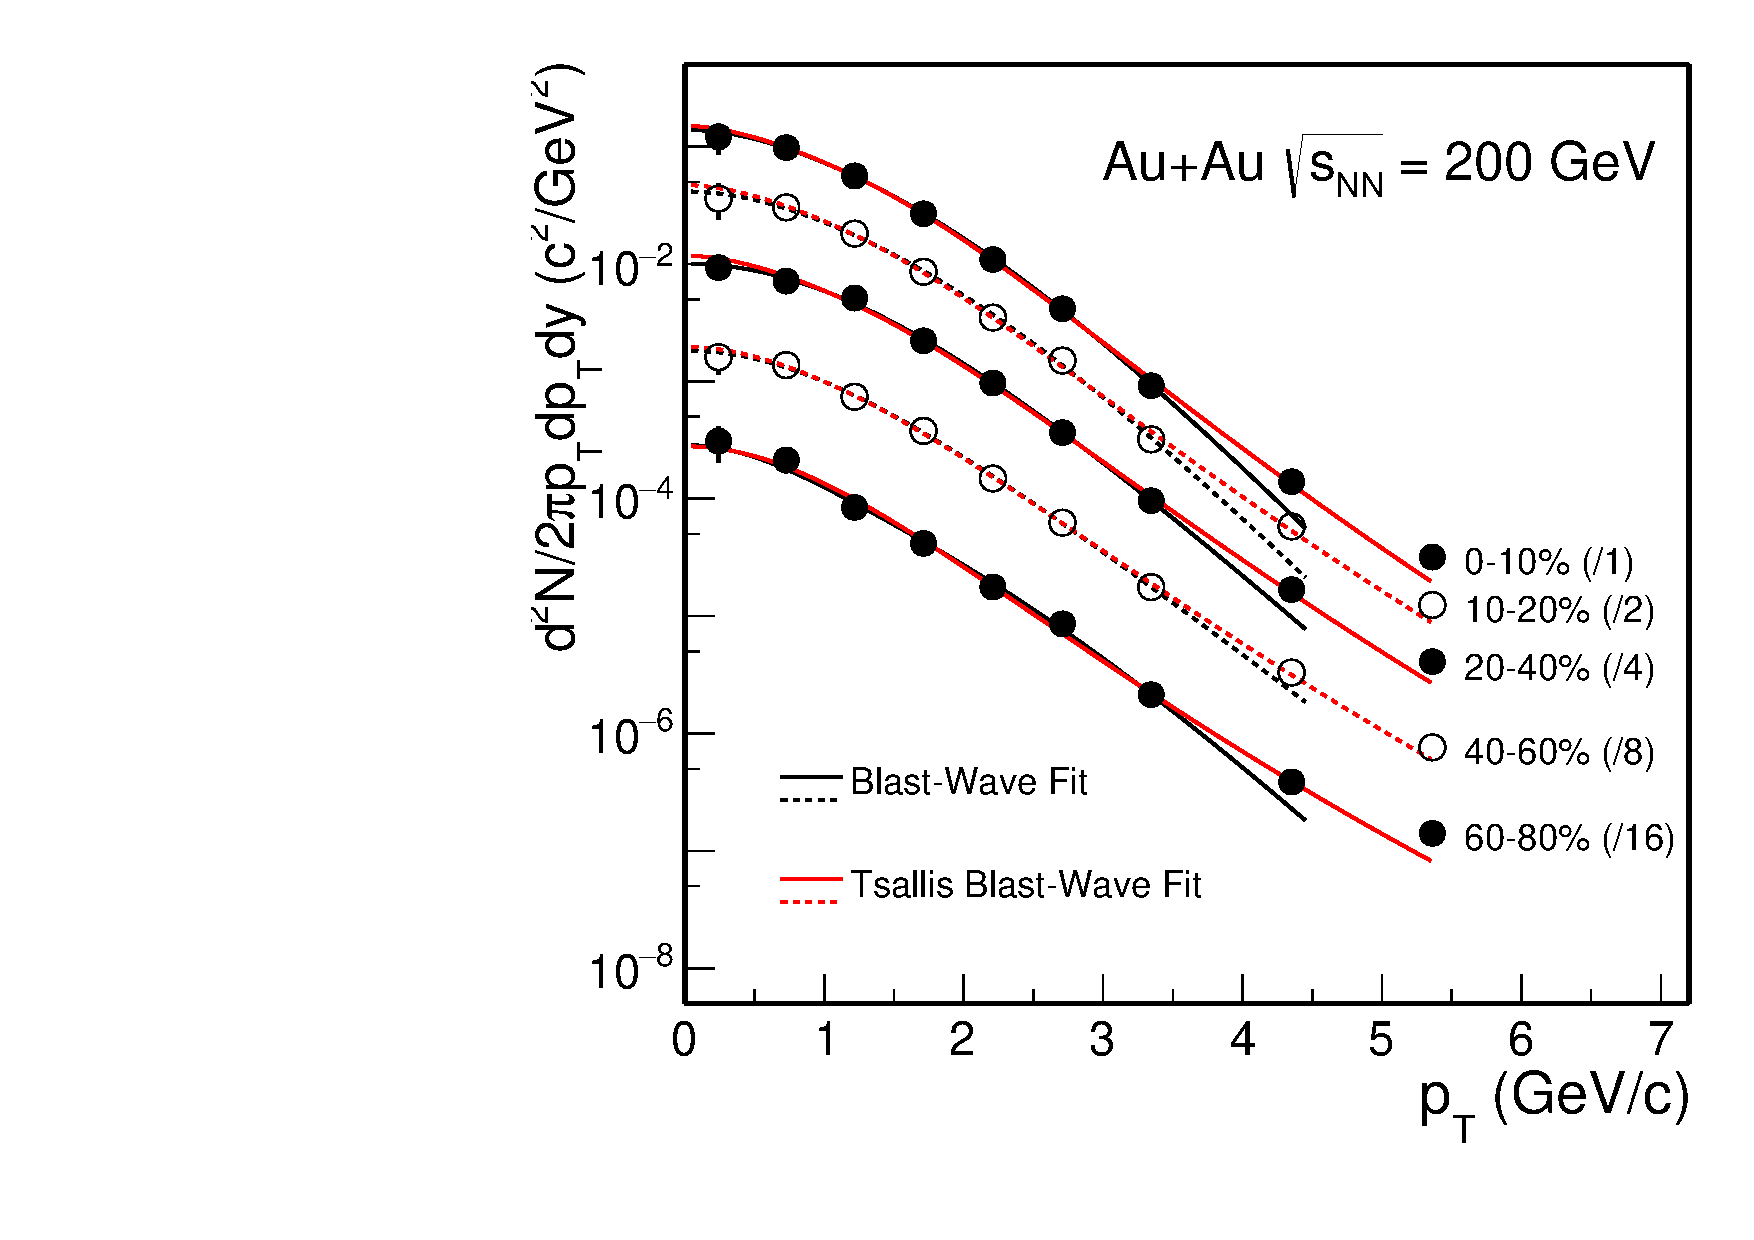
\includegraphics[width=0.68\textwidth]{figure/Run14_D0HFT/BWFit.pdf}
\caption{$D^{0}$ invariant yield at mid-rapidity ($|y|<1$) vs. transverse momentum for different centrality classes in Au + Au collisions at $\sqrt{s_{_{\rm NN}}}$ = 200\,GeV. Solid and dashed black lines depict Blast-Wave function fits.}
\label{Teff_ALL} 
\end{figure}


Blast-wave model is extensively used to study the particle kinetic freeze-out properties. 

Assuming a hard-sphere uniform density particle source with a kinetic freeze-out temperature $T_{\rm kin}$ and a transverse radial flow velocity $\beta$, the particle transverse momentum spectral shape is given by :

\begin{equation}
\frac{dN}{p_{\rm T}dp_{\rm T}} = \frac{dN}{m_{\rm T}dm_{\rm T}} \propto \int_0^R rdr m_{\rm T} I_0\bigg(\frac{p_{\rm T}\sinh\rho}{T_{\rm kin}}\bigg) K_1\bigg(\frac{m_{\rm T}\cosh\rho}{T_{\rm kin}}\bigg)
\end{equation}

where $\rho = \tanh^{-1}\beta$, and $I_0$ and $K_1$ are the modified Bessel functions. The flow velocity profile is taken as

\begin{equation}
\beta = \beta_{\rm S}\left(\frac{r}{R}\right)^{n}
\end{equation}

where $\beta_{\rm S}$ is the maximum velocity at the surface and $r/R$ is the relative radial position in the thermal source. The choice of $R$ only affects the overall spectrum magnitude while the spectrum shape constrains the three free parameters $T_{\rm kin}$, $\langle\beta\rangle=2/(2+n)\beta_{\rm S}$ and $n$.


To account for the degree of non-equilibrium, Tsallis statistics has been introduced into the Blast-wave model with an additional parameter $q-1$, and the Blast-Wave distribution can be modified as

\begin{equation}
\frac{dN}{m_{\rm T}dm_{\rm T}} \propto m_{\rm T}\int_{-Y}^{+Y}\cosh(y)dy \int_{-\pi}^{+\pi} d\phi \int_0^R rdr \bigg(1+\frac{q-1}{T_{\rm kin}}\big(m_{\rm T}\cosh(y)\cosh(\rho)-p_{\rm T}\sinh(\rho)\cos(\phi)\big)\bigg)^{\textstyle -\frac{1}{q-1}}
\end{equation}

In the limit of $q\rightarrow 1$, the TBW distribution returns to the regular Blast-Wave one. The new Tsallis Blast-Wave (TBW) model has been used to fit the RHIC light and strange hadron spectra and it shows nice description of these particle spectra up to 3 GeV/$c$.



\subsection{\label{result:RCP}Nuclear Modification Factor - $R_{\rm CP}$ and  $R_{\rm AA}$}

\begin{figure}
\centering
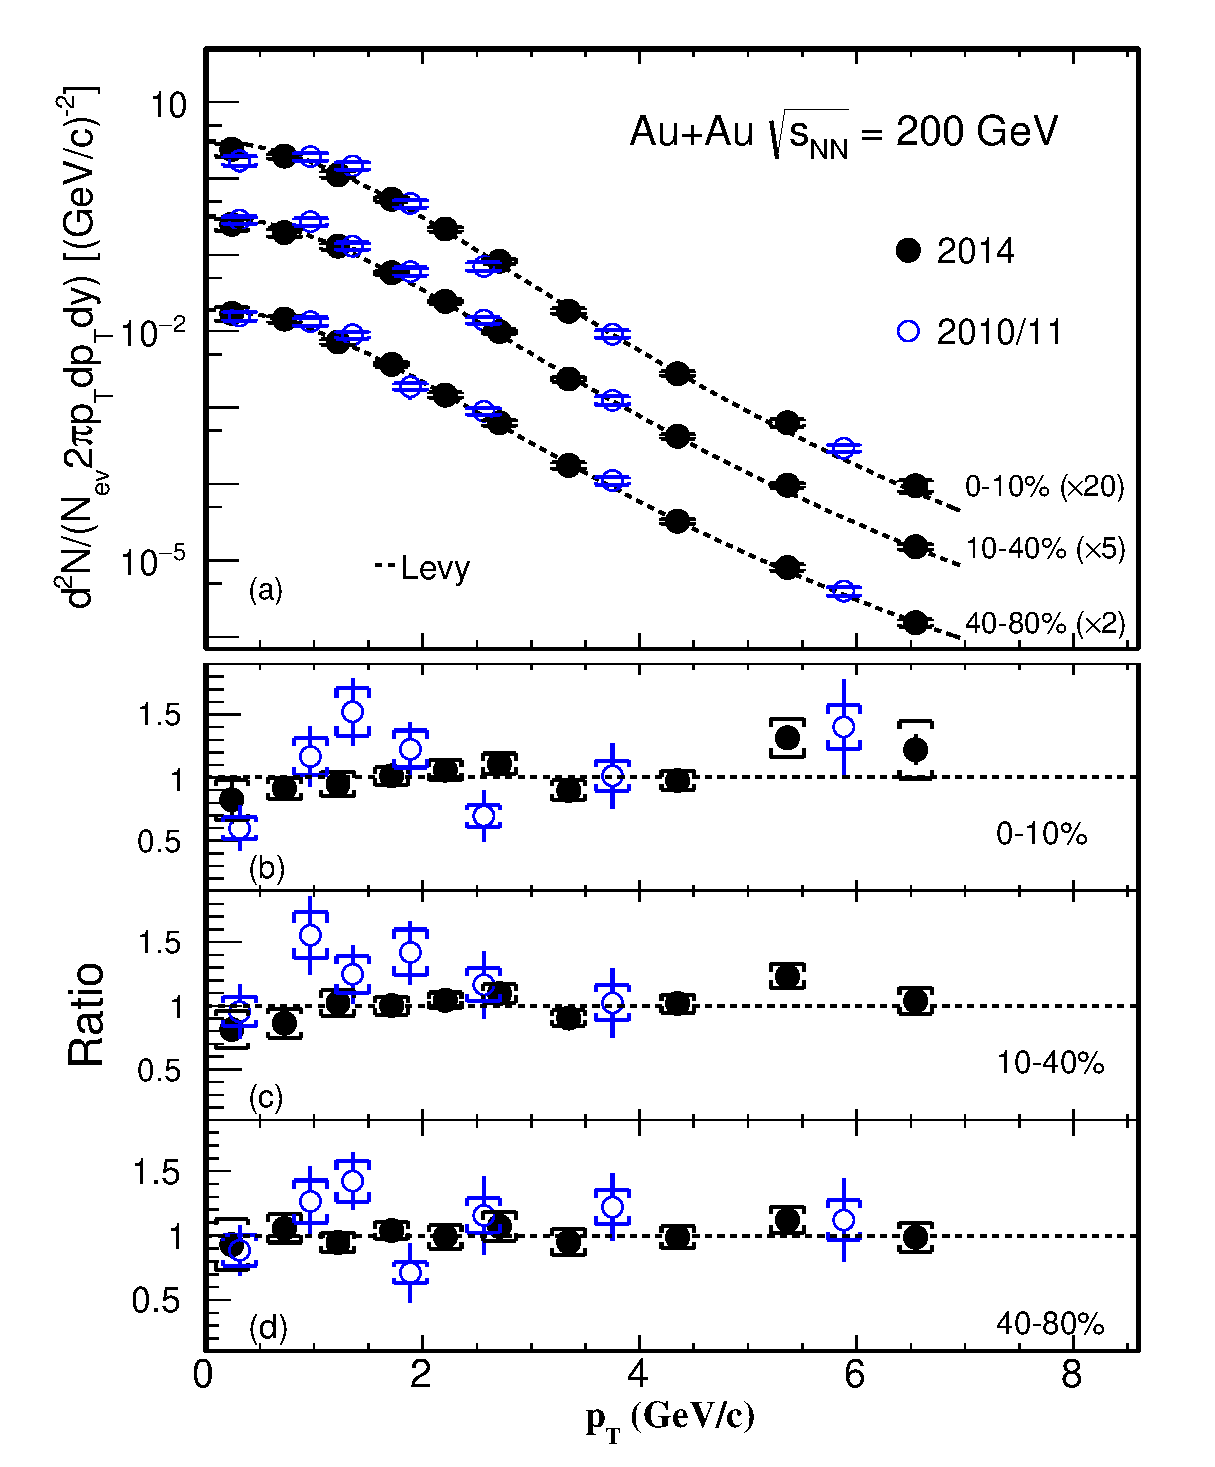
\includegraphics[width=0.68\textwidth]{figure/Run14_D0HFT/D0_compareSpectra_run10.eps}
\caption{$D^{0}$ spectra compare with the run10/11 for different centrality classes in Au + Au collisions.}
\label{D0_compareSpectra_run10} 
\end{figure}

To calculate the $R_{AA}$, we need the p+p baseline measurements. Here, the baseline measurement was from STAR Run09 p+p results. It was combined of $D^0$ and $D^{*}$ measurement with consider the $p_T$ dependence of the $D^*$/$D^0$ ratio. It's kind of different compare to the previous publish result, but we just keep the same as the new run10/11 PRL erratum to select the p+p baseline. Details please find in the erratum note. Here we just want to clarify how the baseline wa and systematic uncertainty was chosen and calculated.

% The central value for p+p result was from the fitted Levy function. As can see, the levy function can describe the measured data quite well. In the whole $p_T$ range, we quote the 1 $\sigma$ band from the fitting as the systematic uncertainties source. For the unmeasured $p_T$ range, say $p_T <$ 1GeV and $>$ 6 GeV, together with the measured range, we have a consistent procedures to add an additional source from the different fitting functions. As can see in the low $p_T$ range, we have run12 preliminary results, the data do not favor power-law shape. Even though without run12 preliminary results, the pythia also do not favor the power-law. So in the low $p_T$ region (<$1 GeV$), we quote the different between levy and BW to consider as the additional systematic uncertainty source. The larger one between 1$\sigma$ band and Levy-BW difference was considered as the systematic uncertainty. In the high $p_T$ range, with our current knowledge, we can't drop those function shapes. So instead of just consider levy and BW, we also include power-low in the high $p_T$ rang, quote the maximum difference as the systematic source. The plots shown in Fig.~\ref{pp_baseLine1} and Fif.~\ref{pp_baseLine2}.

The central value for p+p result was from the fitted Levy function. As can see, the levy function can describe the measured data quite well. In the whole $p_T$ range, we quote the 1 $\sigma$ band from the fitting as the systematic uncertainties source. Due to the constrains from the function shape, the 1$\sigma$ band is kind of smaller compare to the data uncertainties in the measured pt range, but the error band in the unmeasured range is huge. For the unmeasured $p_T$ range, say $p_T <$ 1GeV and $>$ 6 GeV, together with the measured range, we have a consistent procedures to add an additional source from the different fitting functions. This is kind of systematic source from our limited knowledge of the spectra shapes. As can see we also have run12 preliminary results can be used as guidance spectra. In the low $p_T$ and high $p_T$ region (<$1 GeV$ and >$6 GeV$), we quote the different between levy and BW, difference between levy and powlaw to consider as the additional systematic uncertainty source. The plots shown in Fig.~\ref{pp_baseLine1} and Fif.~\ref{pp_baseLine2} are the p+p base lines. 

Fig.~\ref{pp_baseLine_ratio} and Fif.~\ref{pp_baseLine_ratio_3} are the p+p spectra divided to the levy functions. Red points were from run9 publish result while the Black ones are from run12. The band present the 1$\sigma$ fitting uncertainty for Fig.~\ref{pp_baseLine_ratio} while Fig.~\ref{pp_baseLine_ratio} also including the additional systematic source from other functions as described above.

\begin{figure}[htbp]
\begin{minipage}[htbp]{0.47\linewidth}
\centering
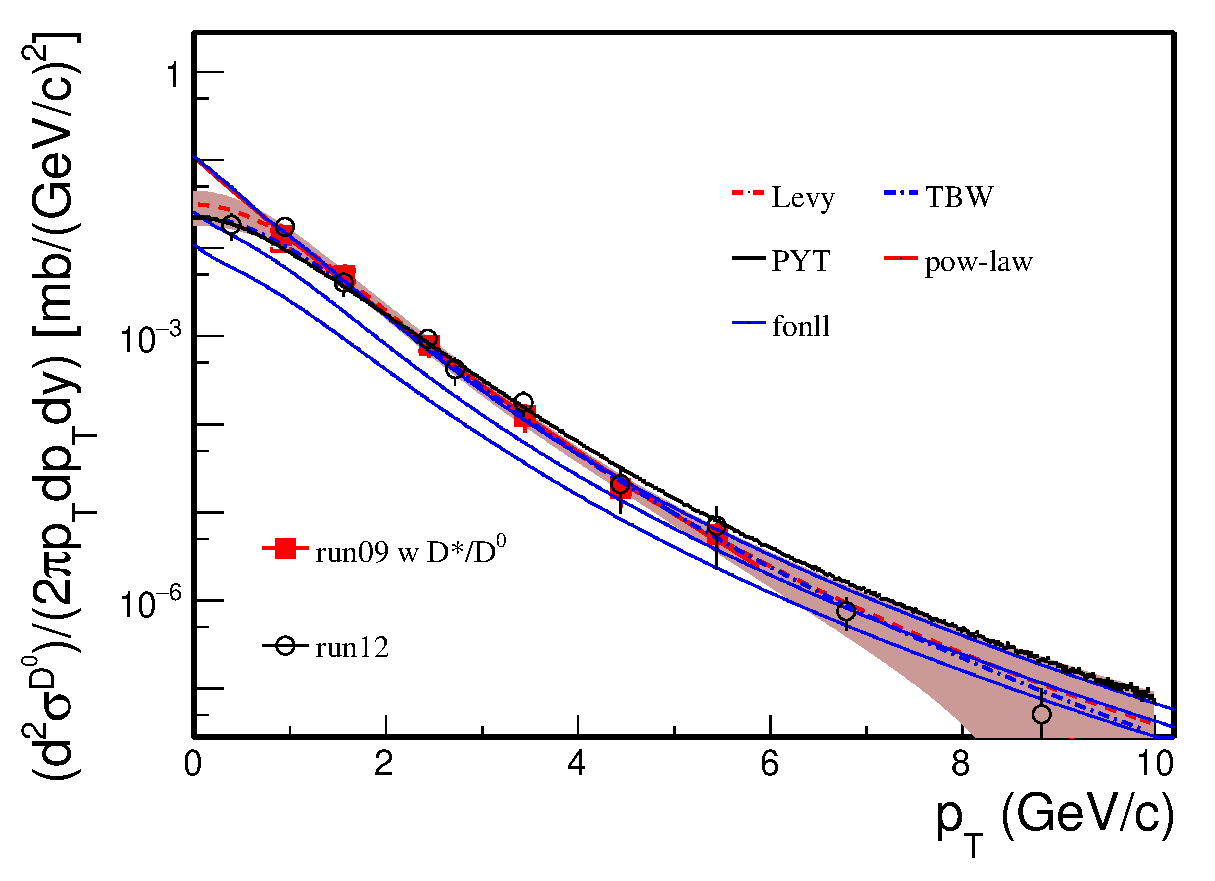
\includegraphics[width=1.0\textwidth,angle=0]{figure/Run14_D0HFT/pp_baseLine1.eps}
\caption{Run09 $D^{0}$ and $D^*$ from p+p collisions fitted with the levy function, power low function, Blast Wave function, PYTHIA shape and also FONLL shape used for the baseline and systematic uncertainty calculations. \label{pp_baseLine1}}
\end{minipage}
\hfill
\begin{minipage}[htbp]{0.47\linewidth}
\centering
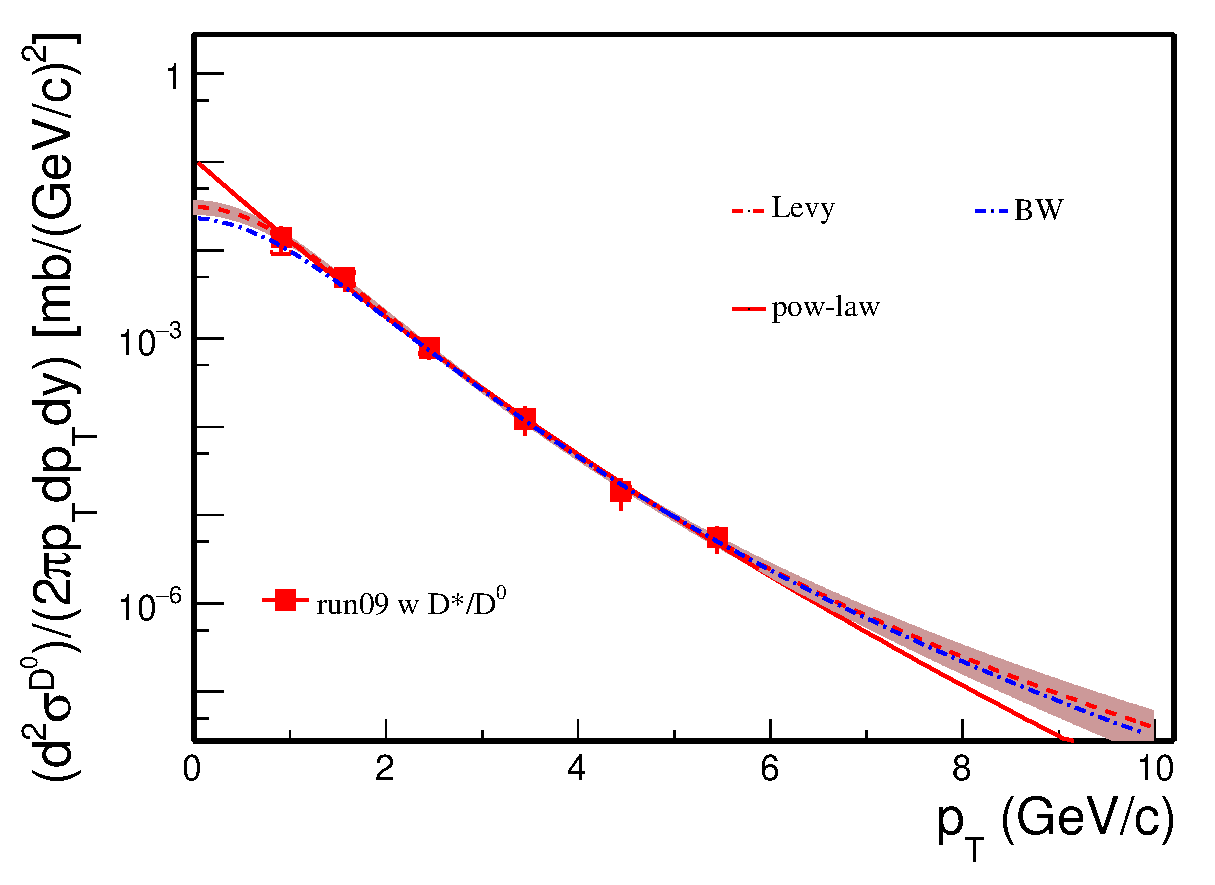
\includegraphics[width=1.0\textwidth,angle=0]{figure/Run14_D0HFT/pp_baseLine2.eps}
\caption{Run09 $D^{0}$ and $D^*$ from p+p collisions fitted with the levy function, power low function, Blast Wave function which is actually used for the systematic uncertainty calculations. \label{pp_baseLine2}}
\end{minipage}
\end{figure}

\begin{figure}[htbp]
\begin{minipage}[htbp]{0.47\linewidth}
\centering
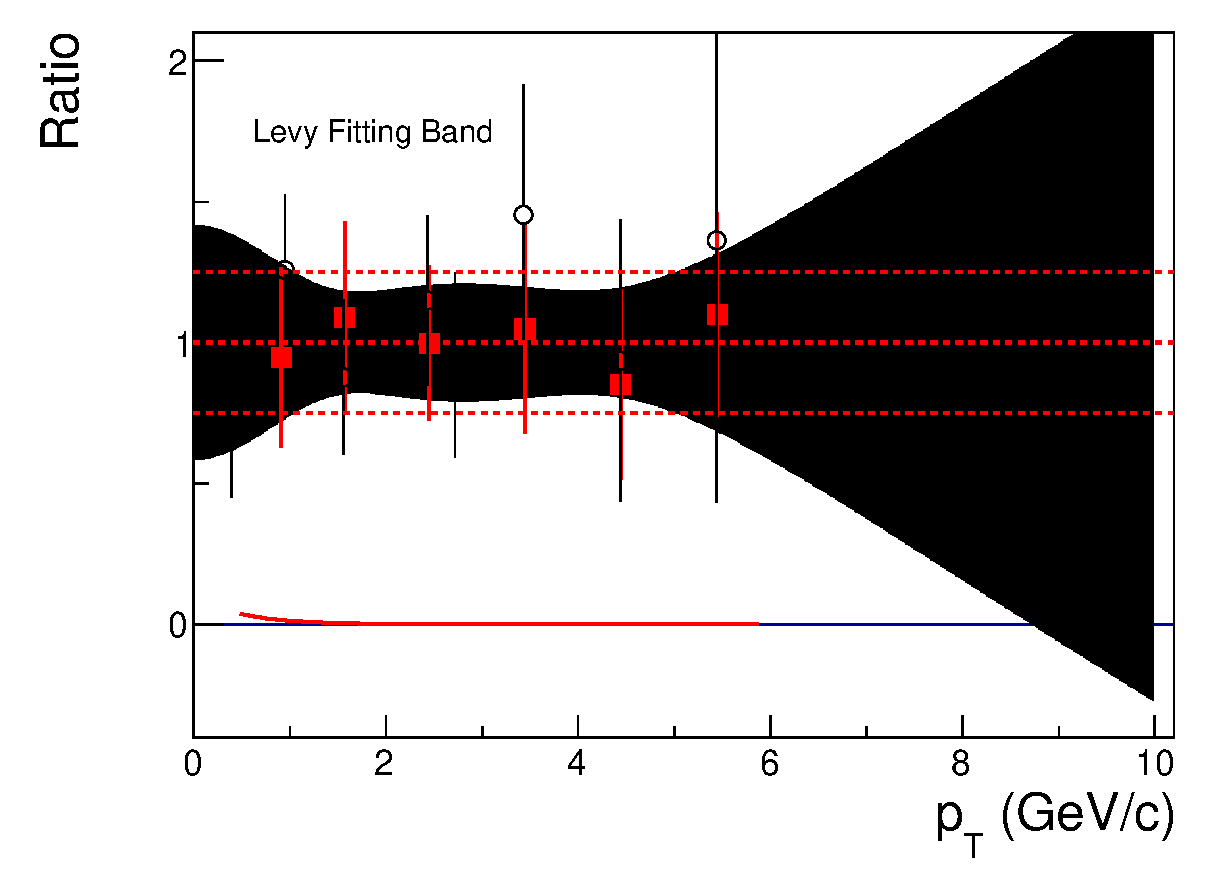
\includegraphics[width=1.0\textwidth,angle=0]{figure/Run14_D0HFT/pp_baseLine_Ratio.eps}
\caption{Run09 $D^{0}$ and $D^*$ (red) run12 (black) from p+p collisions divided to the levy function. The band present the 1$\sigma$ fitting uncertainty. \label{pp_baseLine_ratio}}
\end{minipage}
\hfill
\begin{minipage}[htbp]{0.47\linewidth}
\centering
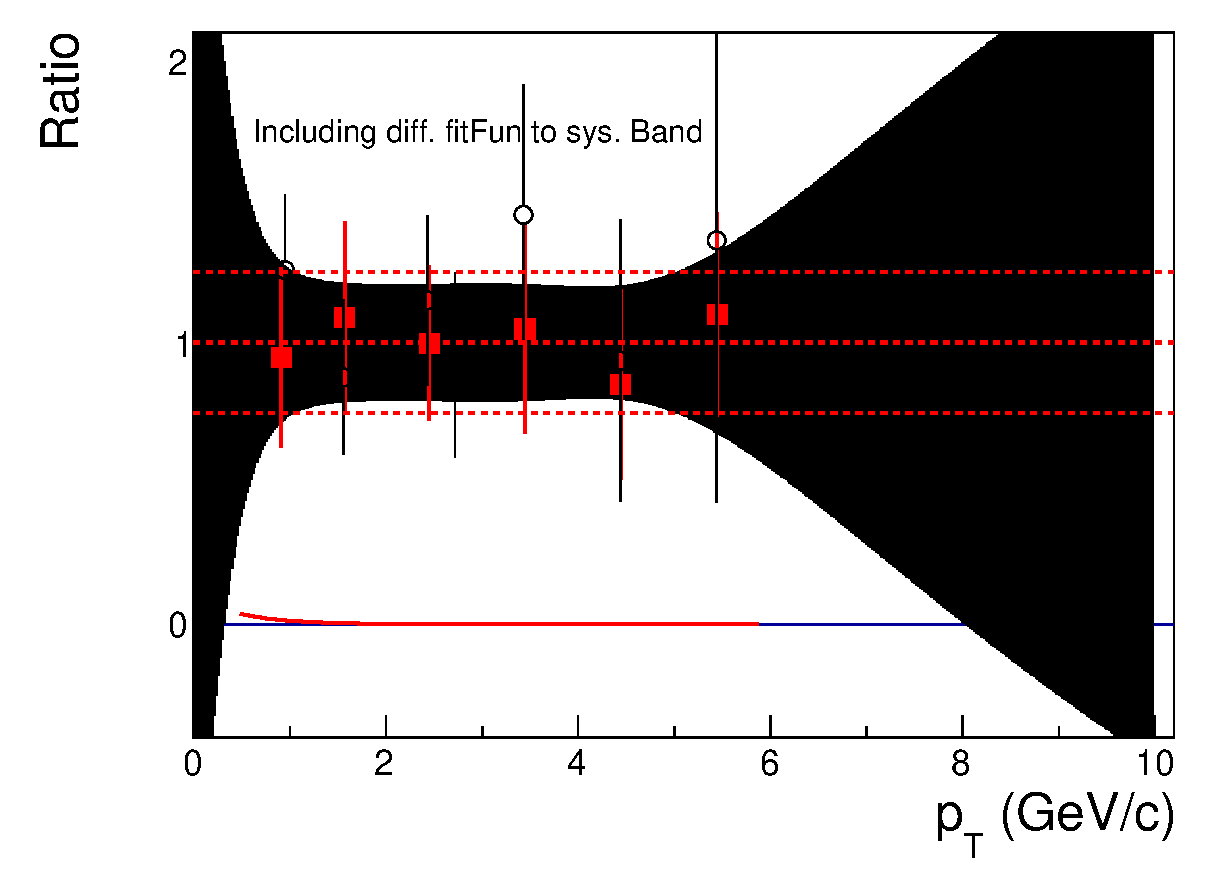
\includegraphics[width=1.0\textwidth,angle=0]{figure/Run14_D0HFT/pp_baseLine_Ratio3.eps}
\caption{Run09 $D^{0}$ and $D^*$ (red) run12 (black) from p+p collisions divided to the levy function. The band present the 1$\sigma$ fitting uncertainty plus the additional systematic source from other functions as described above. \label{pp_baseLine_ratio_3}}
\end{minipage}
\end{figure}


\begin{figure}
\centering
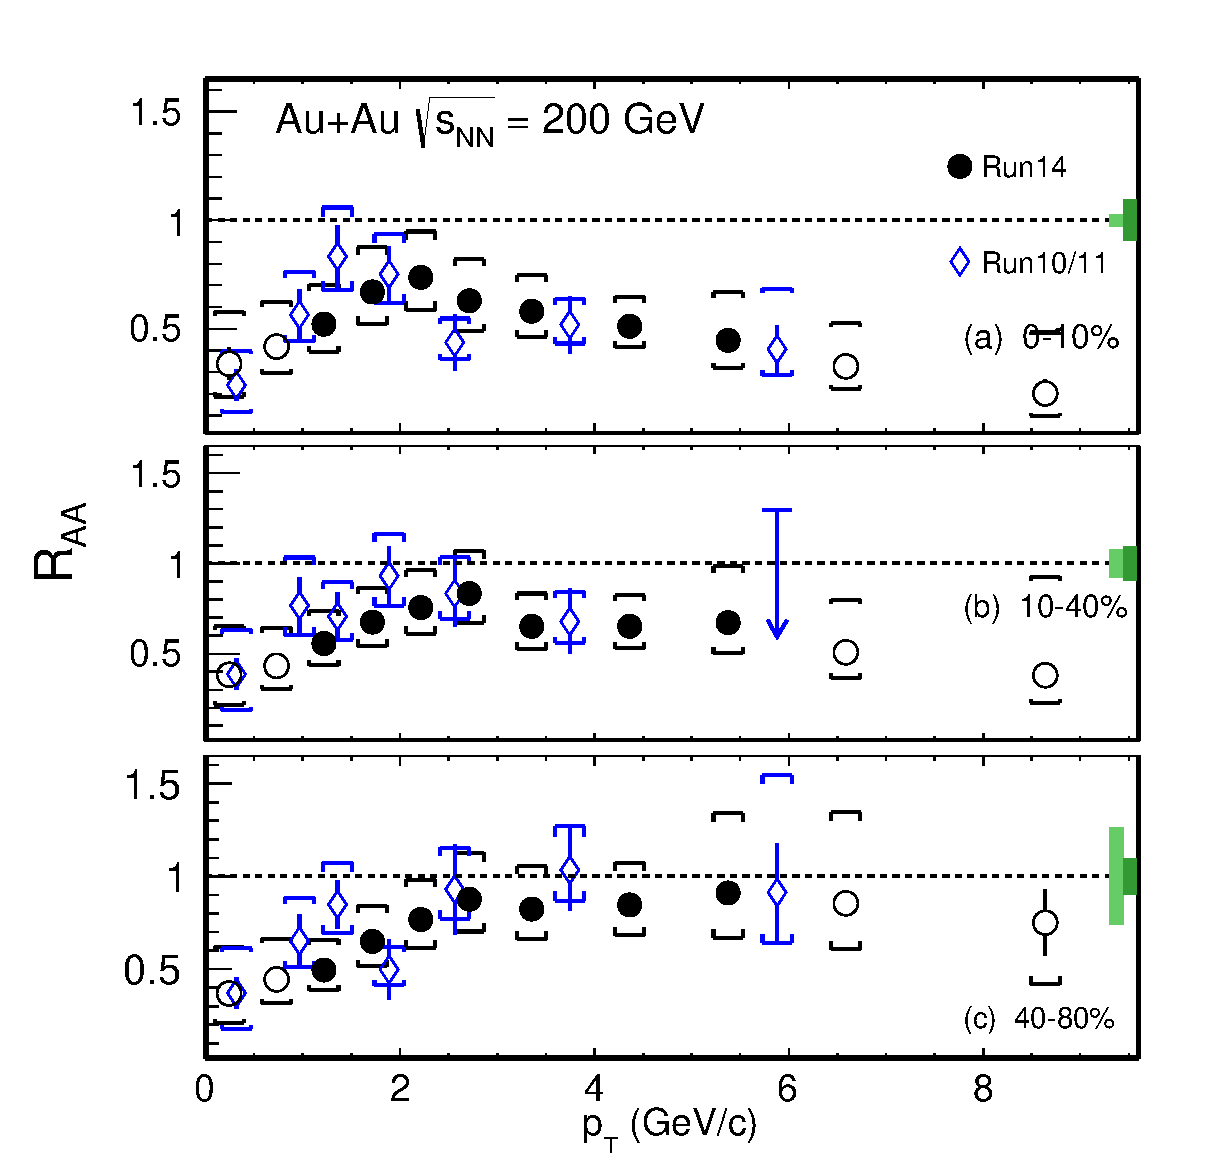
\includegraphics[width=0.68\textwidth]{figure/Run14_D0HFT/D0_RAA.eps}
\caption{$D^{0}$ $R_{\rm AA}$ with the run9 p+p spectrum Ref.[Phys.Rev.D 86(2012)72013] as the reference for different centrality classes in Au + Au collisions.}
\label{D0_RAA} 
\end{figure}

\begin{figure}
\centering
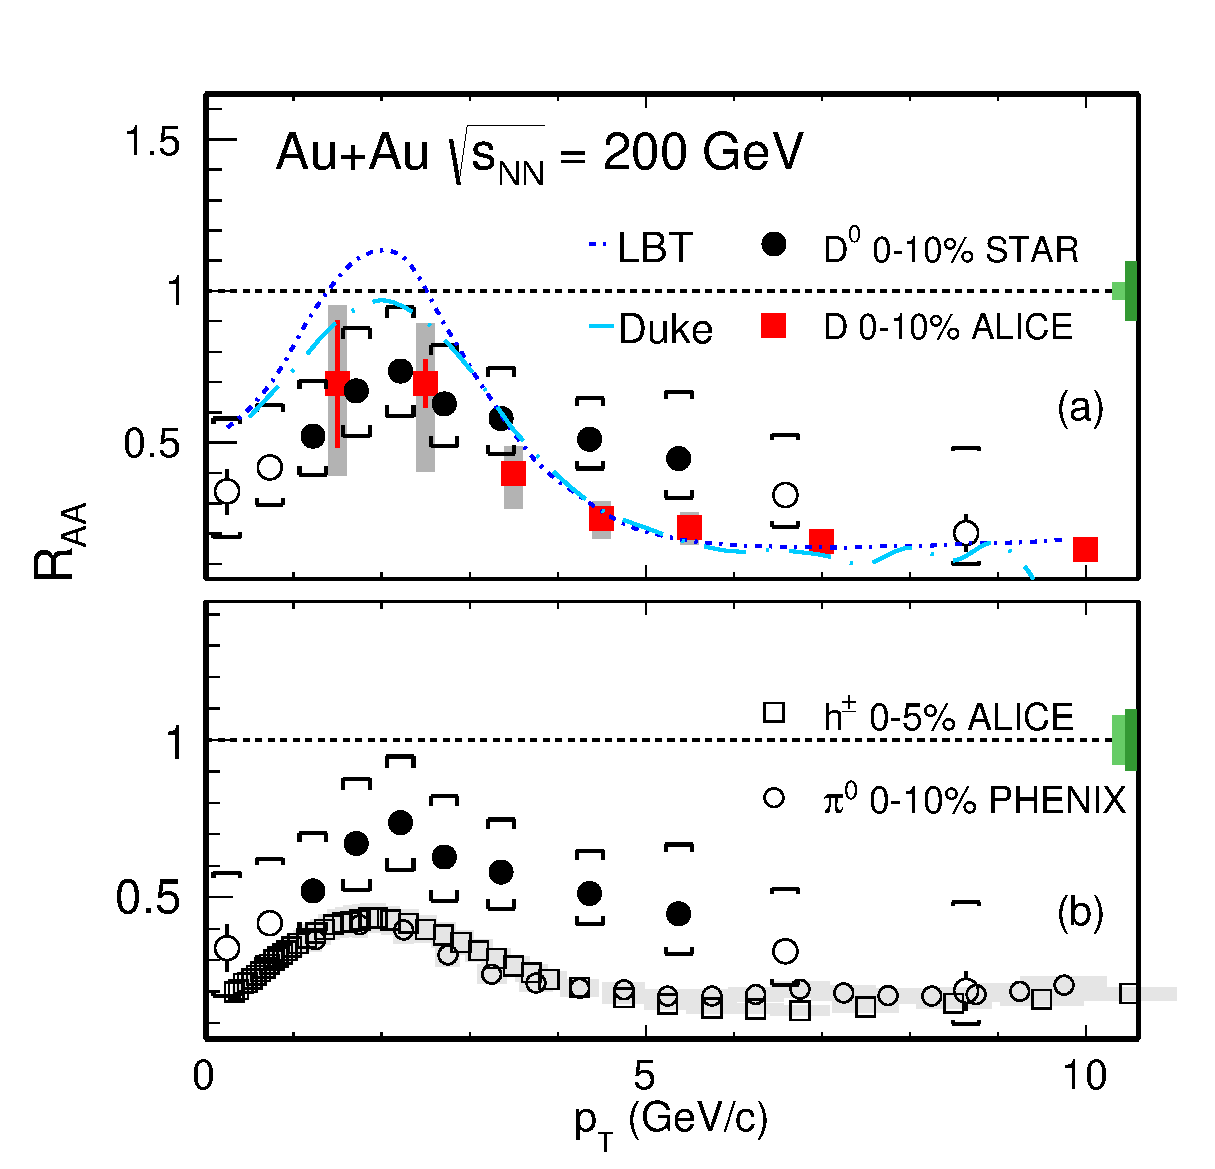
\includegraphics[width=0.68\textwidth]{figure/Run14_D0HFT/D0_RAA_LHC.eps}
\caption{$D^{0}$ $R_{\rm AA}$ in the most central collisions at 0-10\% compared to that of D meson from ALICE and charged hadron from ALICE and $\pi^0$ from APHENIX.}
\label{D0_RAA_LHC} 
\end{figure}

\begin{figure}
\centering
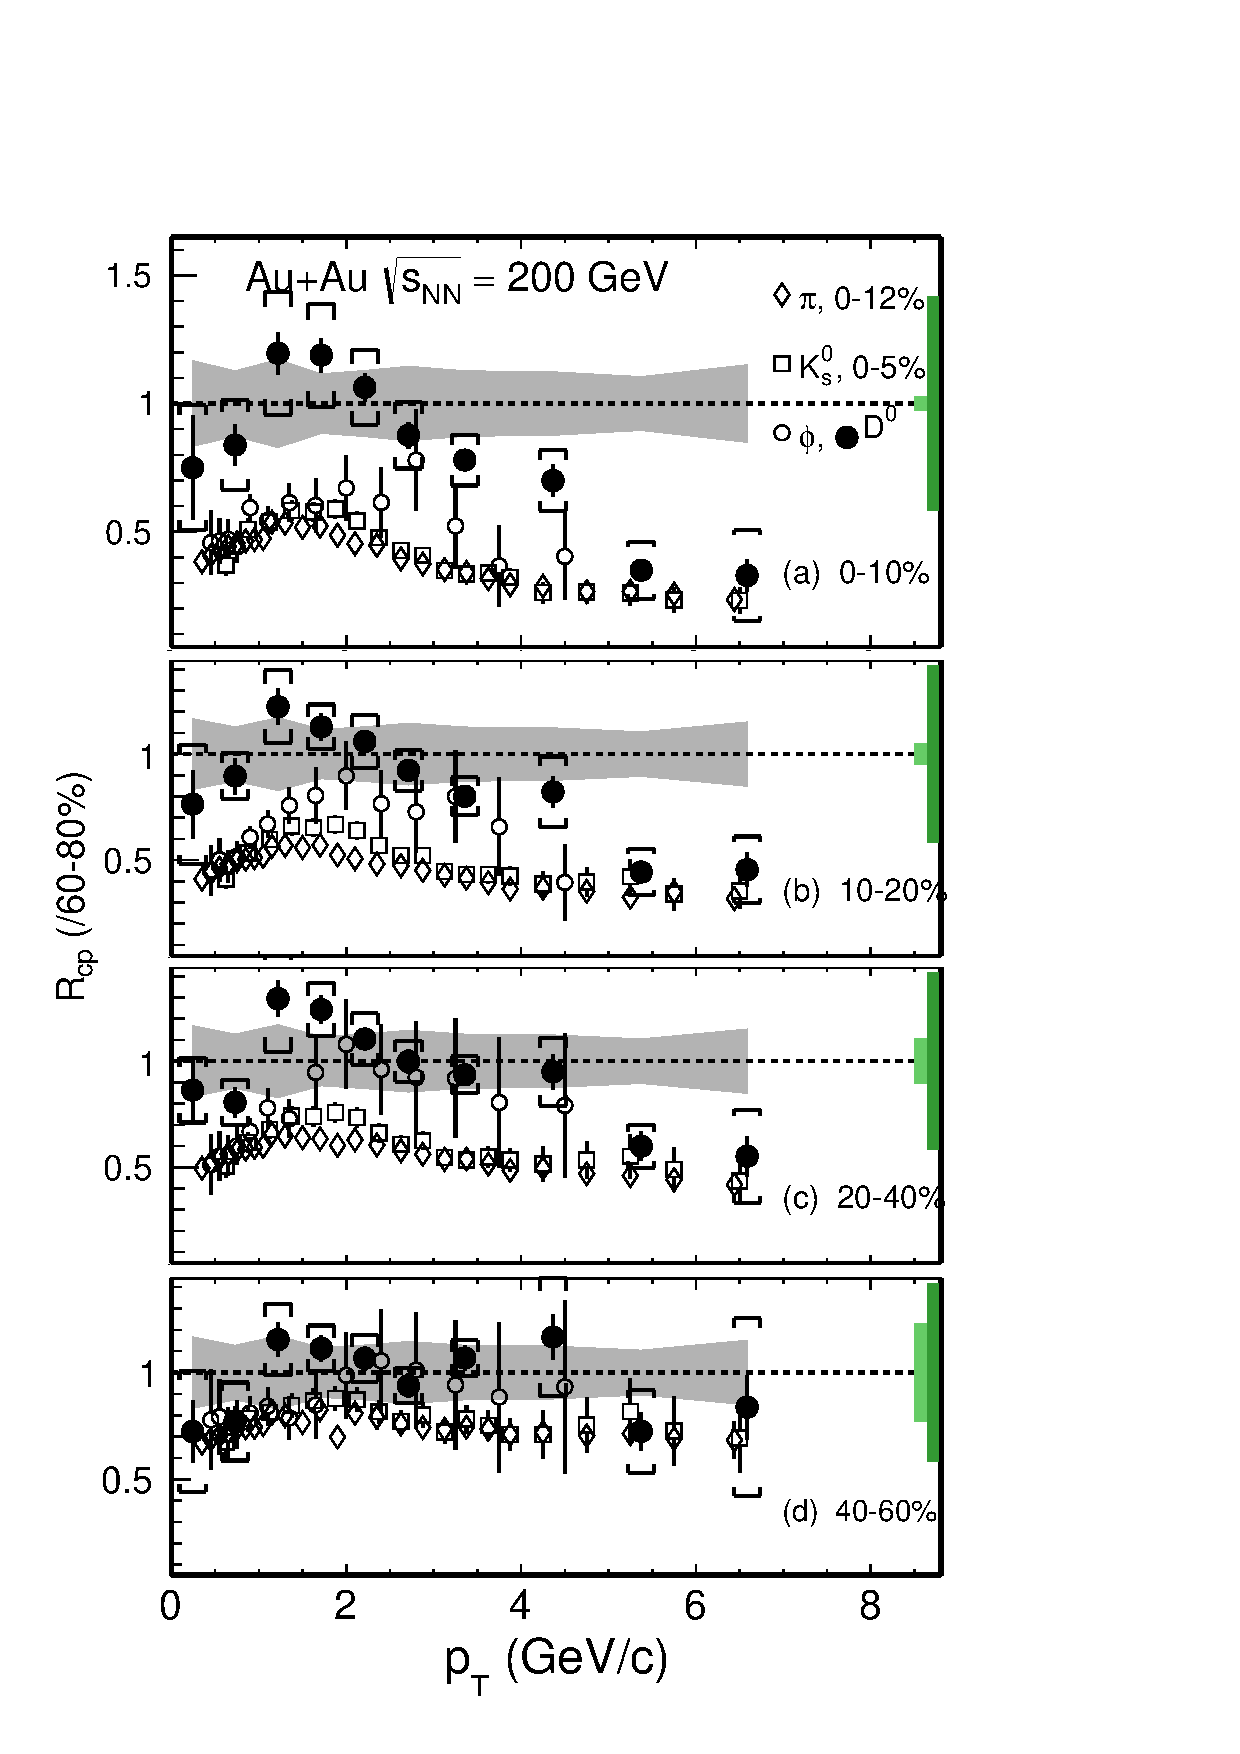
\includegraphics[width=0.68\textwidth]{figure/Run14_D0HFT/D0_Rcp1.pdf}
\caption{$D^{0}$ $R_{\rm CP}$ with the 60--80\% spectrum as the reference for different centrality classes in Au + Au collisions at $\sqrt{s_{_{\rm NN}}}$ = 200\,GeV compared to that of other light and strange mesons ($\pi^{\pm}$, $K^0_{S}$ and $\phi$). The statistical and systematic uncertainties are shown as error bars and brackets on the data points. The grey bands around unity depict the systematic uncertainty due to vertex resolution correction, mostly from the 60--80\% reference spectrum. The light and dark green boxes on the right depict the normalization uncertainty in determining the $N_{\rm bin}$.}
\label{D0_Rcp} 
\end{figure}

Fig.~\ref{D0_Rcp} shows the calculated $R_{\rm CP}$ for several different centralities including 0-10\%, 10-20\%, 20-40\% and 40-60\%, here the base line is the most peripheral collisions 60-80\%. In the top panel, the band around unity was the vertex contribution for the systematic uncertainties from the most peripheral collisions at 60-80\%, these contribution also applied for the other $R_{\rm CP}$ centrality species. As a comparison, there are also three samples shown for pions, $K_{s}$ and $\phi$ in the top 10\% centrality. Bottom panels show the similar $R_{\rm CP}$ but for the other centralities.

\begin{figure}
\centering
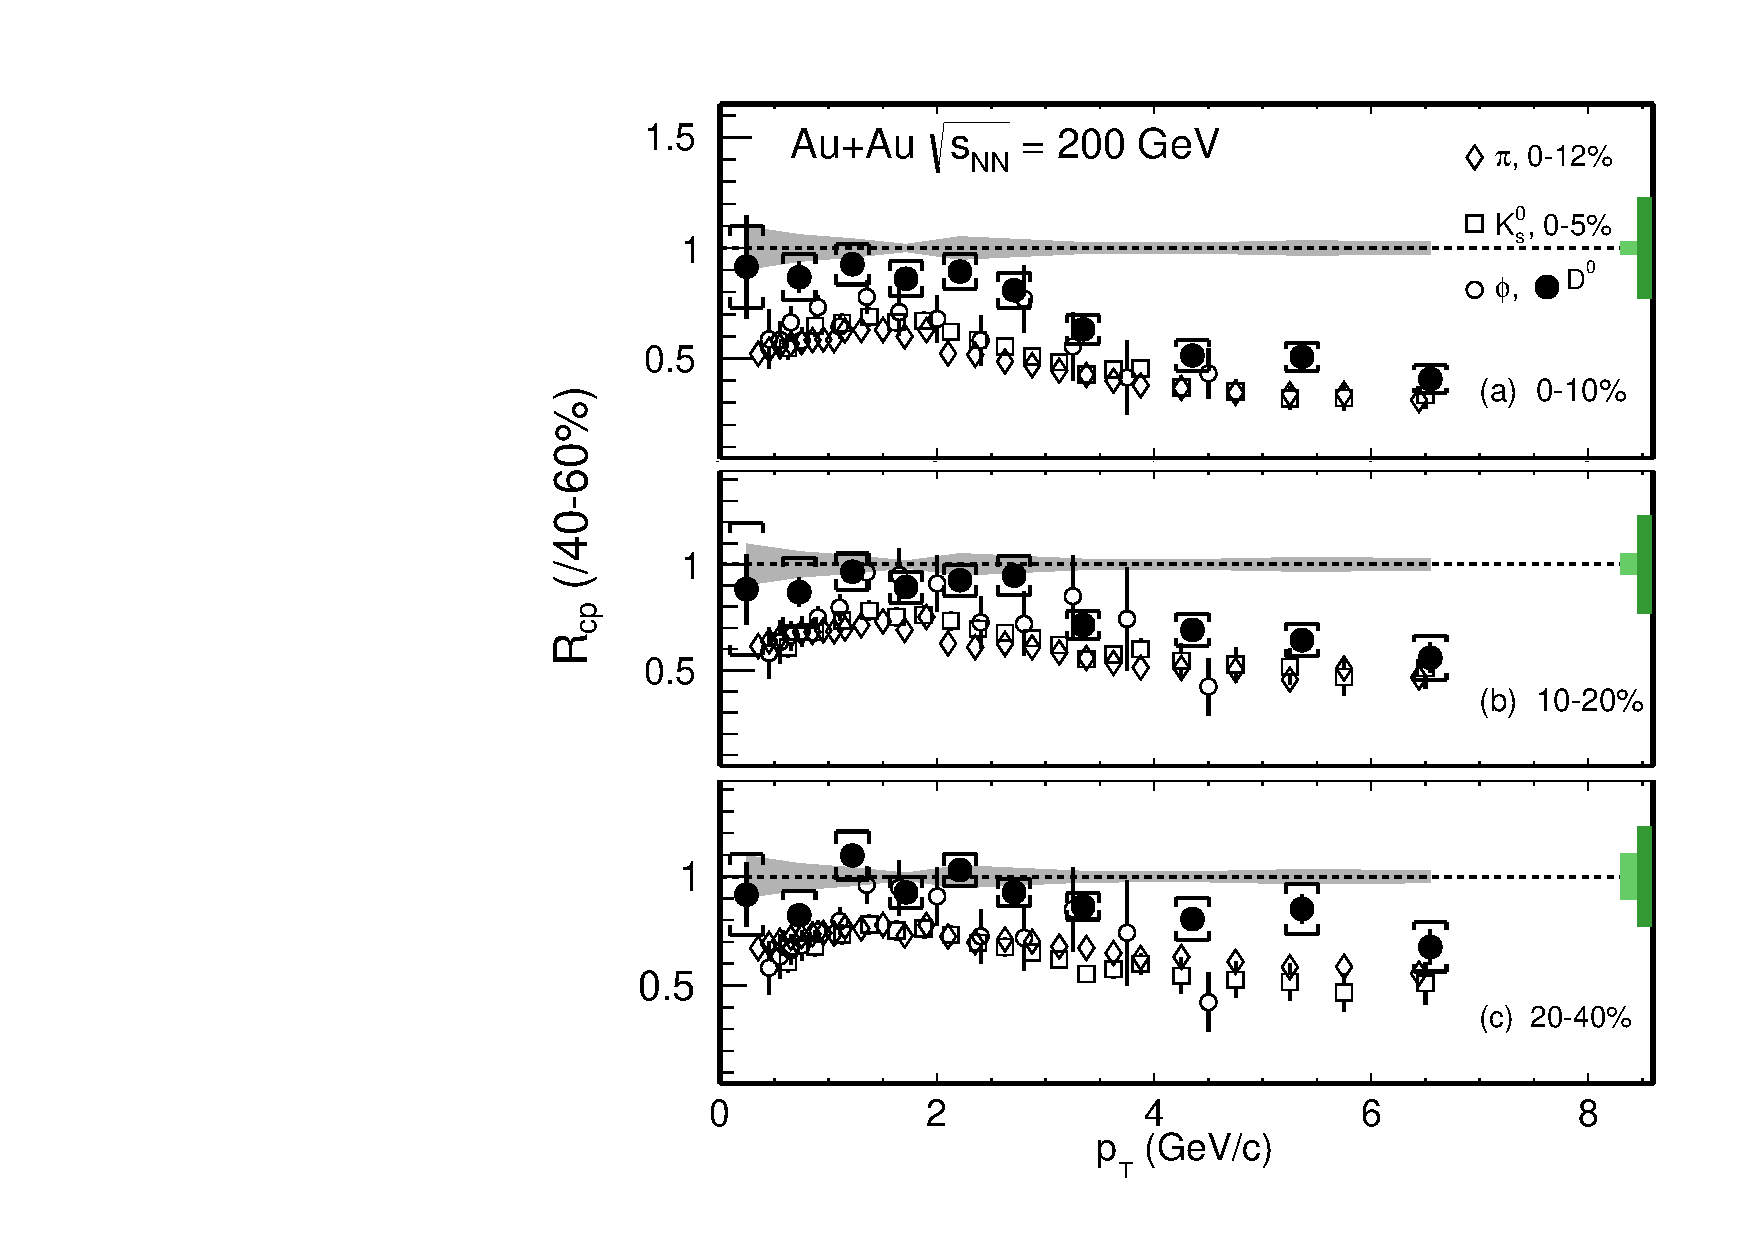
\includegraphics[width=0.68\textwidth]{figure/Run14_D0HFT/D0_Rcp2.pdf}
\caption{$D^{0}$ $R_{\rm CP}$ with the 40--60\% spectrum as the reference for different centrality classes in Au + Au collisions at $\sqrt{s_{_{\rm NN}}}$ = 200\,GeV compared to that of other light and strange mesons ($\pi^{\pm}$, $K^0_{S}$ and $\phi$). The statistical and systematic uncertainties are shown as error bars and brackets on the data points. The grey bands around unity depict the systematic uncertainty due to vertex resolution correction, mostly from the 40--60\% reference spectrum. The light and dark green boxes on the right depict the normalization uncertainty in determining the $N_{\rm bin}$.}
\label{D0_Rcp2} 
\end{figure}

Fig.~\ref{D0_Rcp2} shows the similar $R_{\rm CP}$ for different centralities as Fig.~\ref{D0_Rcp}, but the base line here is change to 40-80\% centralities. The band around unity in the top panel was the vertex contribution for the systematic uncertainties from 40-80\% centralities, also applied to the other bottom $R_{\rm CP}$ centrality species. As a comparison, pions, $K_{s}$ and $\phi$ in several centralities are plotted on the correlated panel.

\begin{figure*}
\centering
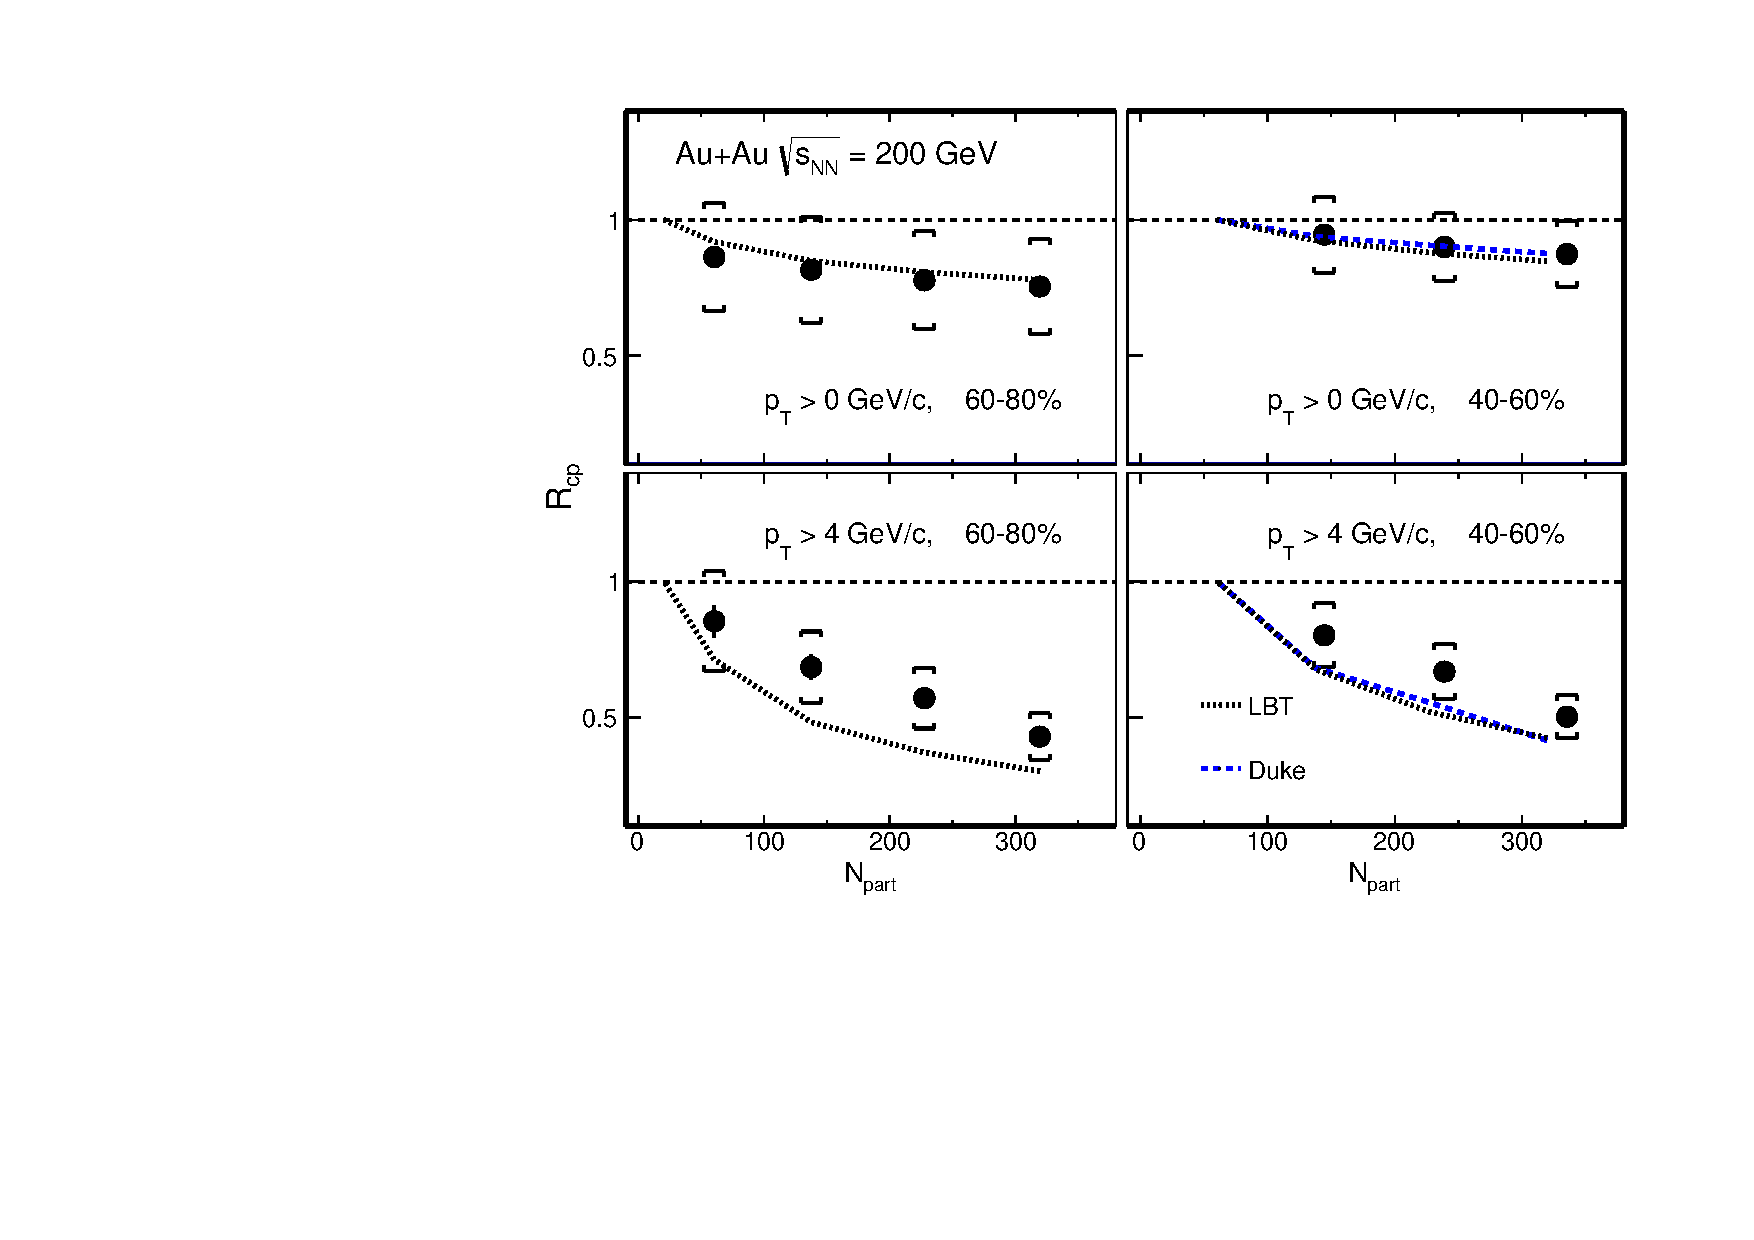
\includegraphics[width=0.8\textwidth]{figure/Run14_D0HFT/Rcp_Nbin_D0.pdf}
\caption{$D^{0}$ $R_{\rm CP}$ vs. $N_{\rm bin}$ in Au + Au collisions.}
\label{Rcp_Nbin_D0} 
\end{figure*}


\begin{figure}
\centering
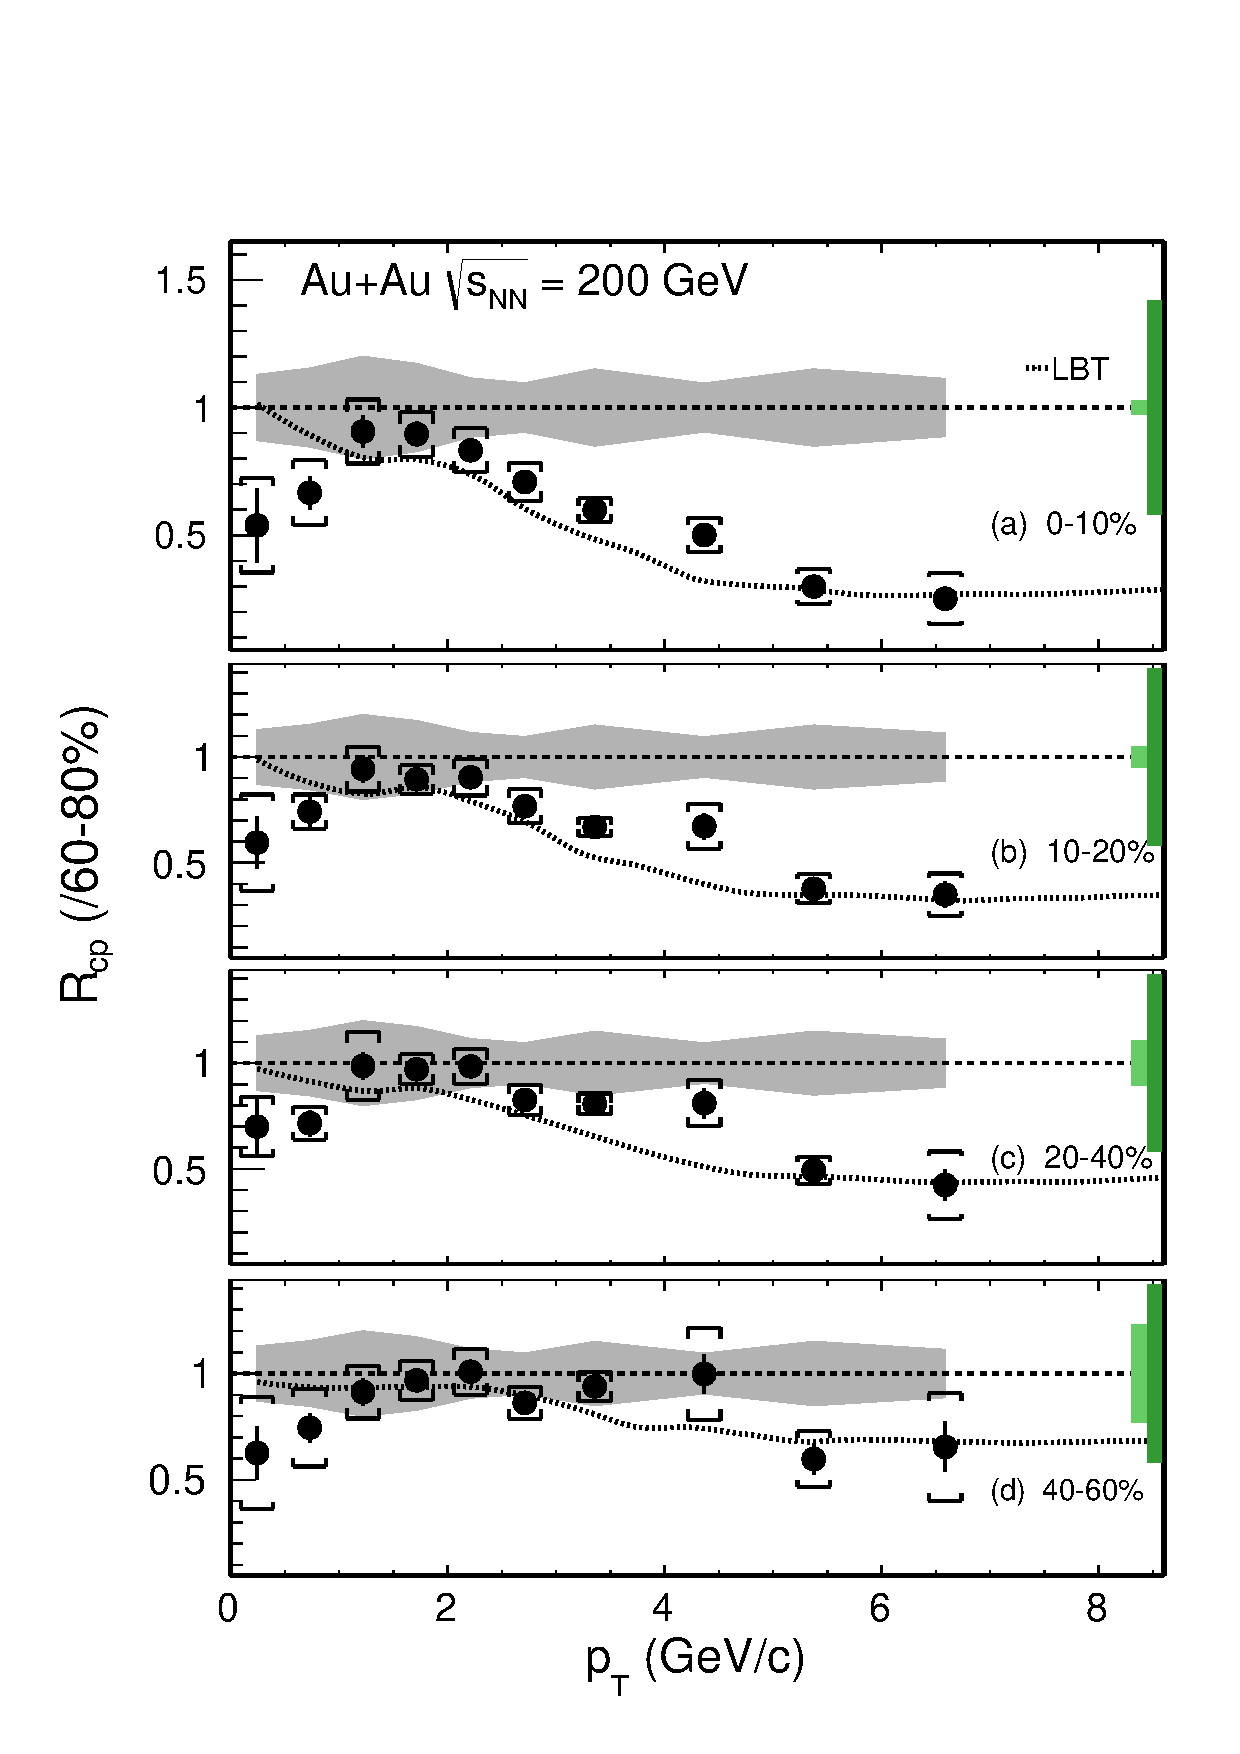
\includegraphics[width=0.68\textwidth]{figure/Run14_D0HFT/D0_Rcp11.pdf}
\caption{$D^{0}$ $R_{\rm CP}$ with the 60--80\% spectrum as the reference for different centrality classes in Au + Au collisions compared to model calculations. The statistical and systematic uncertainties are shown as error bars and brackets on the data points. The grey bands around unity depict the systematic uncertainty due to vertex resolution correction, mostly from the 60--80\% reference spectrum. The light and dark green boxes on the right depict the normalization uncertainty in determining the $N_{\rm bin}$.}
\label{D0_Rcp11} 
\end{figure}

\begin{figure}
\centering
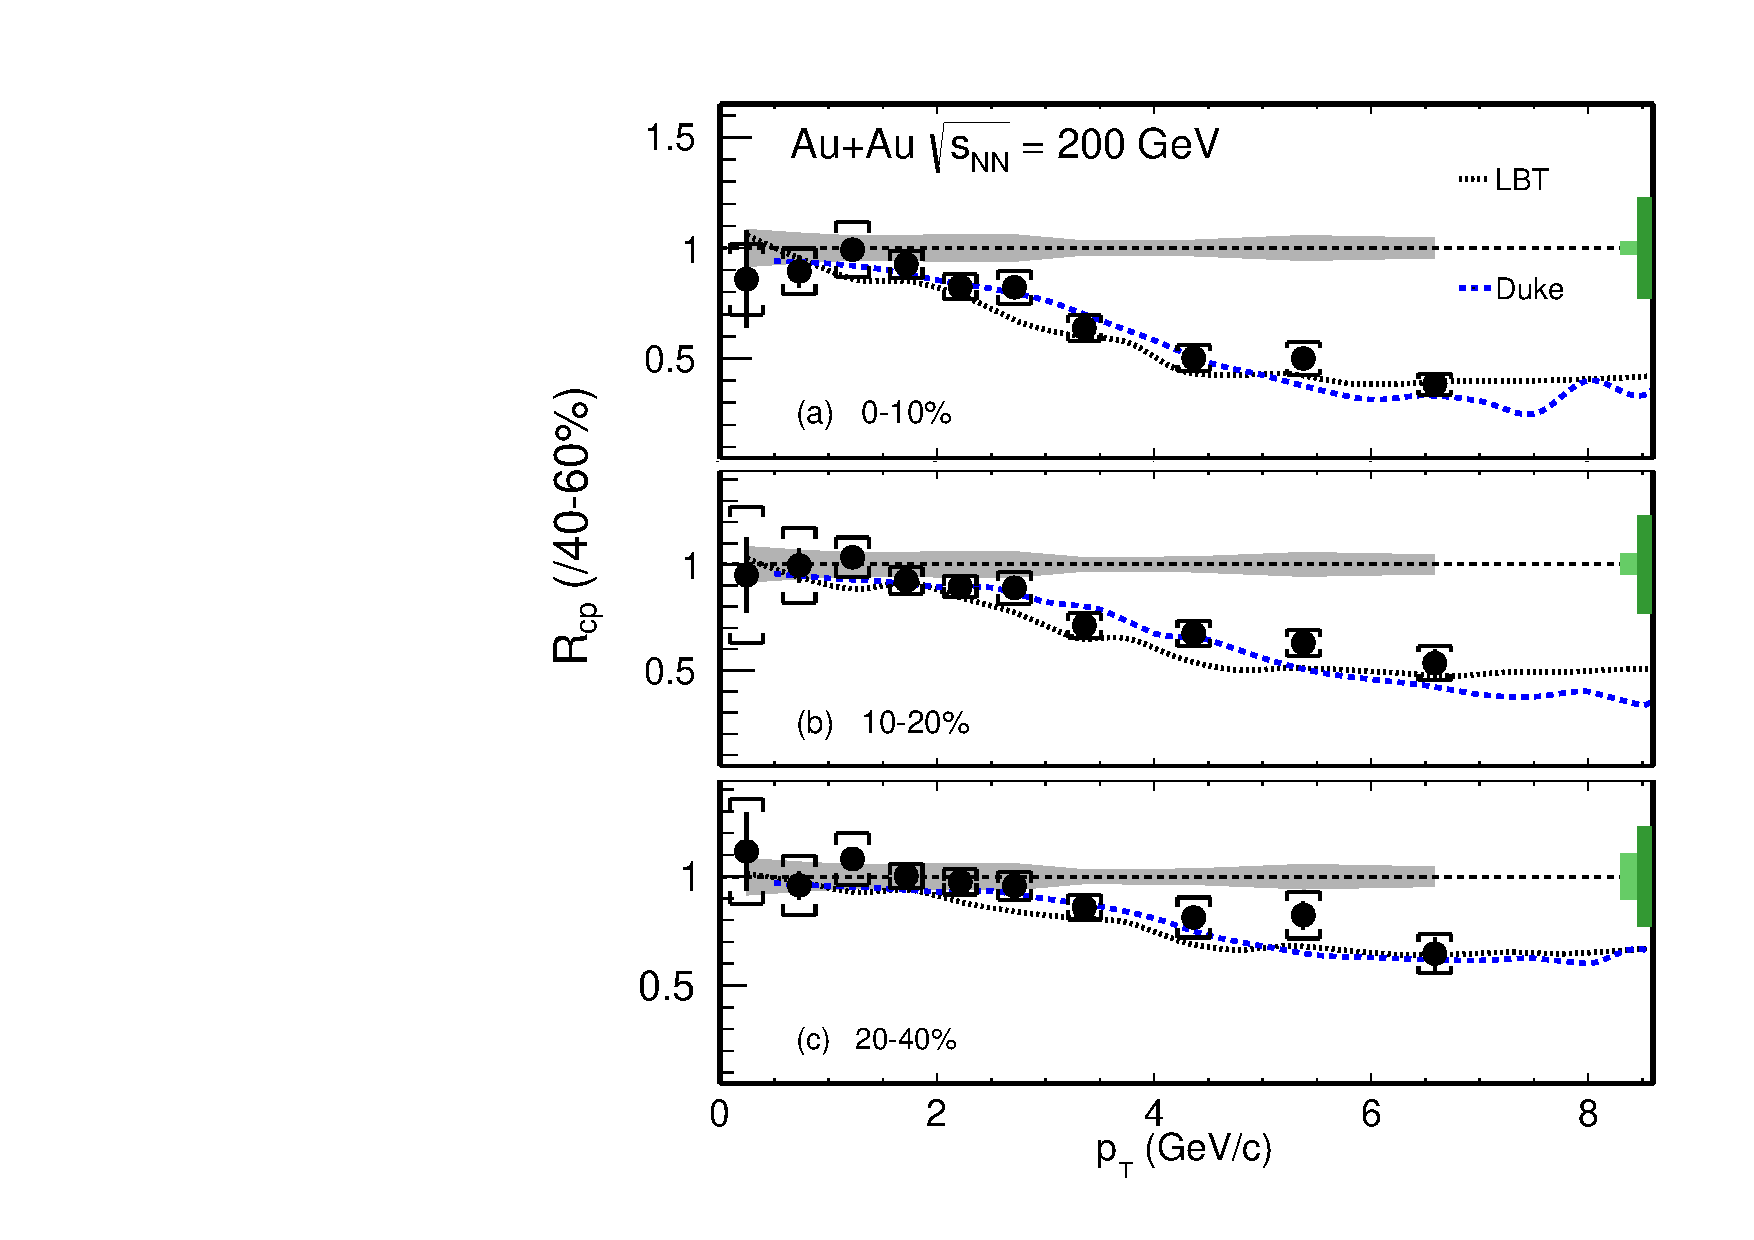
\includegraphics[width=0.68\textwidth]{figure/Run14_D0HFT/D0_Rcp22.pdf}
\caption{$D^{0}$ $R_{\rm CP}$ with the 40--60\% spectrum as the reference for different centrality classes in Au + Au collisions compared to model calculations. The statistical and systematic uncertainties are shown as error bars and brackets on the data points. The grey bands around unity depict the systematic uncertainty due to vertex resolution correction, mostly from the 40--60\% reference spectrum. The light and dark green boxes on the right depict the normalization uncertainty in determining the $N_{\rm bin}$.}
\label{D0_Rcp22} 
\end{figure}

\subsection{\label{D0barD0ratio} $\bar{D^{0}}$ and $D^{0}$ spectra and double ratio}

\begin{figure}
\centering
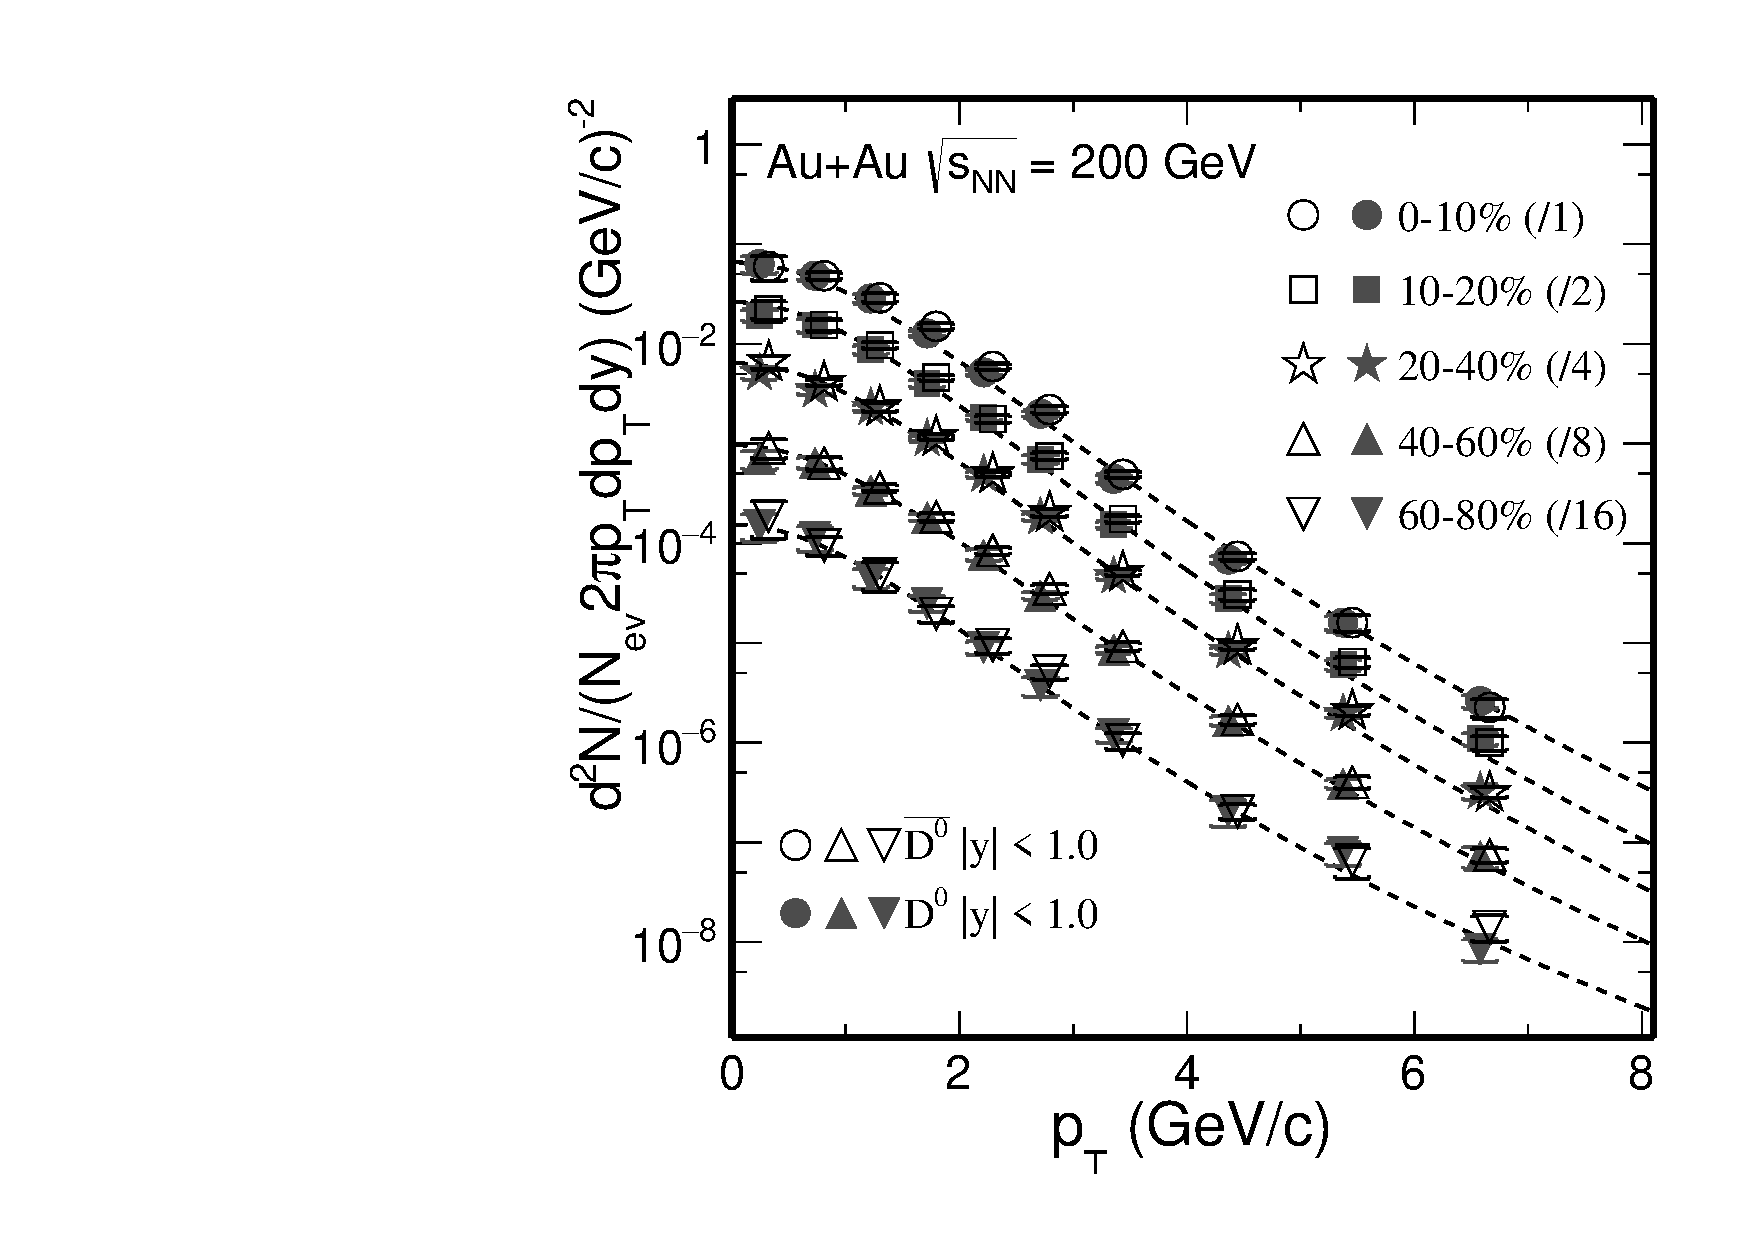
\includegraphics[width=0.68\textwidth]{figure/Run14_D0HFT/D0_spectra_bothposneg.pdf}
\caption{$D^{0}$ and $\bar{D^{0}}$ invariant yield at mid-rapidity ($|y|<1$) vs. transverse momentum for different centrality classes in Au + Au collisions at $\sqrt{s_{_{\rm NN}}}$ = 200\,GeV. Error bars (not visible for many data points) indicate statistical uncertainties and brackets depict systematical uncertainties. Global systematic uncertainties in $B.R.$ and $N_{\rm bin}$ are not plotted. Solid lines depict Levy function fits.}
\label{D0_spectra_bothposneg} 
\end{figure}

\begin{figure}
\centering
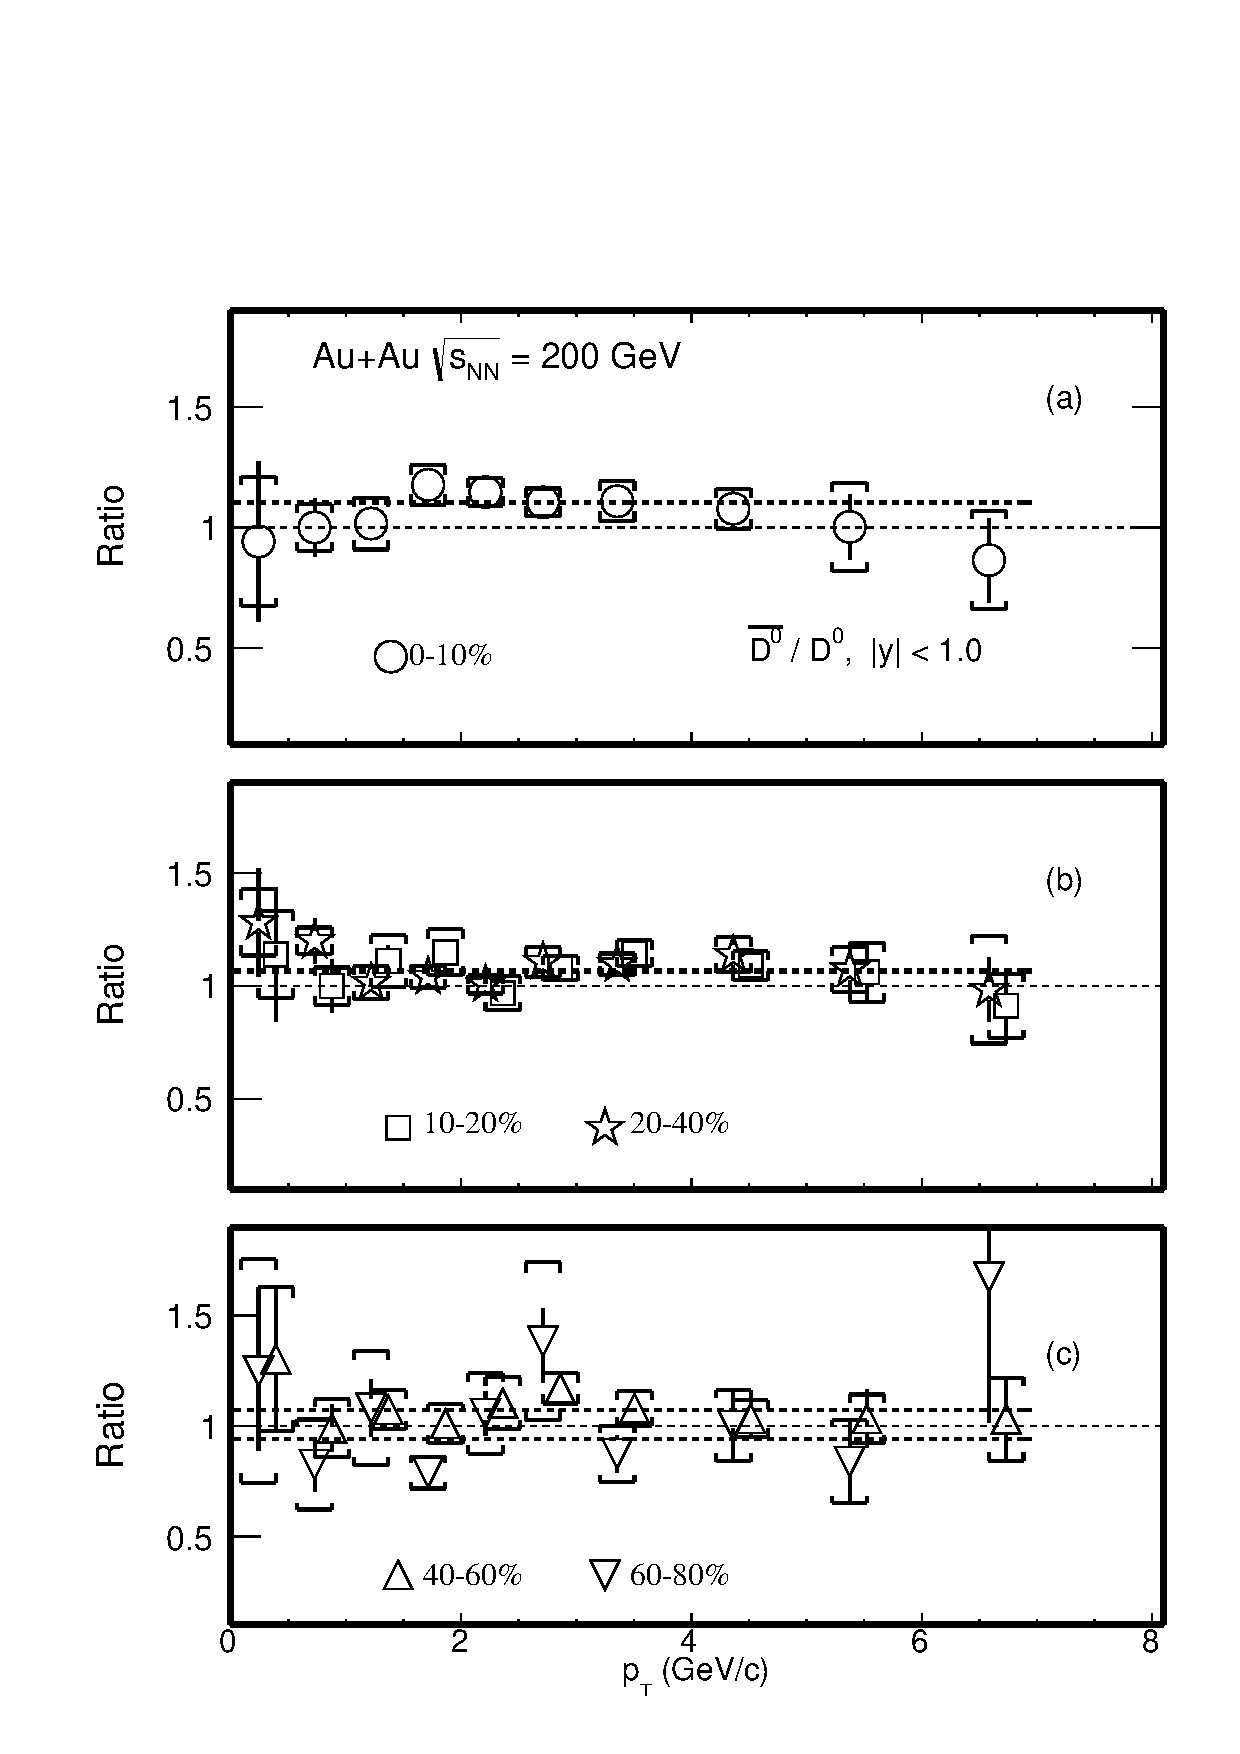
\includegraphics[width=0.68\textwidth]{figure/Run14_D0HFT/D0_spectra_ratioposneg.pdf}
\caption{$\bar{D^{0}}$/$D^{0}$ invariant yield ratio at mid-rapidity ($|y|<1$) vs. transverse momentum for different centrality classes in Au + Au collisions at $\sqrt{s_{_{\rm NN}}}$ = 200\,GeV. Error bars indicate statistical uncertainties and brackets depict systematical uncertainties. Global systematic uncertainties in $B.R.$ and $N_{\rm bin}$ are not plotted. Dashed lines depict a linear function fits.}
\label{D0_spectra_ratioposneg} 
\end{figure}

Fig.~\ref{D0_spectra_bothposneg} shows the $p_{\rm T}$ spectra comparison between $\bar{D^{0}}$ and $D^0$ in 0--10\%, 10--20\%, 20--40\%, 40--60\% and 40--80\% centrality bins. Fig.~\ref{D0_spectra_ratioposneg} shows the $\bar{D^{0}}|$/$D^{0}$ double ratio in the corresponding centrality species. With the current data, there is a hint that the $\bar{D^{0}}$ yield is relative larger than the $D^{0}$ in the most central and mid-central collisions. There could be some physics message behind, since we expect the $\bar{\Lambda_{c}^-}$/$\Lambda_{c}^+$ ratio should be smaller then unity due to the finite baryon density. The total charm quark and anti-charm quark should be conserved since they are created in pair, which results to the measured $\bar{D^0}$ larger than the $D^0$. This could also arise the precise measurements for $D^{+}$/$D^{-}$ and $D_{s}^{+}$/$D_{s}^{-}$ in the future.


\subsection{\label{result:theory}Comparison to Models}

Over the past several years, there have been rapid developments in the theory model calculations 

The Duke model uses a Langevin stochastic simulation to trace the charm quark propagation inside the QGP medium. Both collisional energy loss and radiative energy loss have been included in the calculation and charm quarks are hardronized via a hybrid approach combining both coalescence and fragmentation mechanisms. The bulk medium is simulated using a viscous hydrodynamic evoluation for the QGP evoluation and a hadronic cascade evolution using the UrQMD model. The charm quark in-medium interaction is characterized using a temperature and momentum dependent diffusion coefficient. The medium evoluation parameters have been constrained via a statistical Bayesian analysis by fitting the previous experimental data of $R_{\rm AA}$ and $v_{2}$ of light, strange and charm hadrons. The extracted charm quark spatial diffusion coefficient at zero momentum $2\pi TD_s|_{p=0}$ is about 1--3 near $T_{\rm c}$ and exhibits a positive slope for its temperature dependence above $T_{\rm c}$.

The Linearized Boltzmann Transport (LBT) calculation extends the LBT approach developed before to include both light and heavy flavor parton evoluation in the QGP medium. The transport calculation includes all $2\rightarrow 2$ elastic scattering processes for collisional energy loss and the higher-twist energy loss formalism for medium induced radiative energy loss. It uses the same hybrid approach as in the Duke model for charm quark hadronization. The heavy quark transport is coupled with a 3D viscous hydrodynamic evolution which is tuned for light flavor hadron data. The charm quark spatial diffusion coefficient is estimated via the $2\pi TD_s =8\pi/\hat{q}$ at parton momentum $p = 10$\,GeV/$c$. The $2\pi TD_s$ is $\sim$3 at $T_{\rm c}$ and increases to $\sim$6 at $T = 500$\,MeV.

We compare our measured $R_{\rm CP}$ to several theory model calculations, shown in Fig.~\ref{D0_Rcp11} and Fig.~\ref{D0_Rcp22}. 

\subsection{\label{result:totalCC} Total ccbar cross section}

Relay on the current charm related analysis, there is a nature question regarding on the total charm cross section. So using the current D0, Dpm, Dstar and Lc results and also relay on some theory prediction for the non-measured pt range. The detail slides can be found below: and We are using 10-40\% centrality for this testing.

https://drupal.star.bnl.gov/STAR/system/files/charmCrossSection\_v2.pdf


\begin{figure}[htbp]
\begin{minipage}[htbp]{0.47\linewidth}
\centering
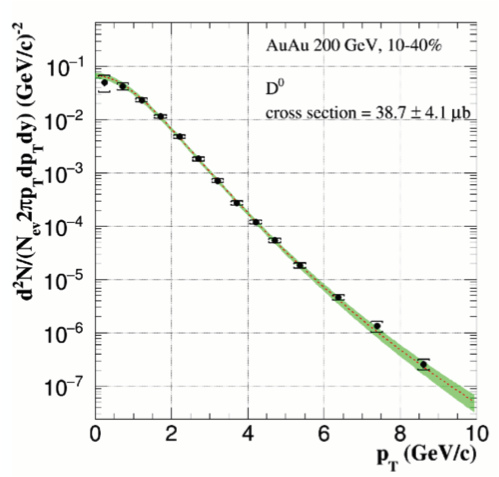
\includegraphics[width=1.0\textwidth,angle=0]{figure/Run14_D0HFT/ccx_1.png}
\caption{$D^{0}$ with the 10--40\% spectrum in Au + Au collisions fitted with the levy function and power low function used for the cross section calculation, then take the difference between two functions as the systematic uncertainties. \label{ccx_1}}
\end{minipage}
\hfill
\begin{minipage}[htbp]{0.47\linewidth}
\centering
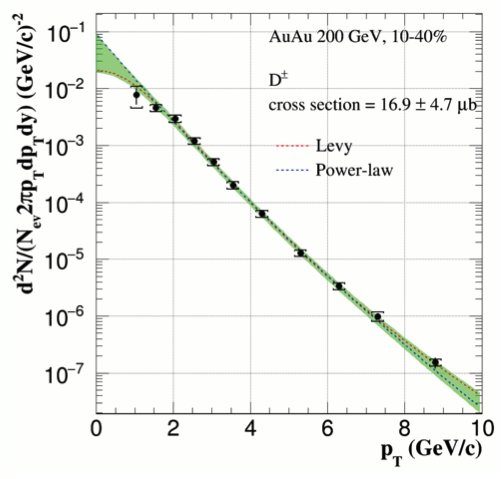
\includegraphics[width=1.0\textwidth,angle=0]{figure/Run14_D0HFT/ccx_2.png}
\caption{$D^{\pm}$ with the 10--40\% spectrum in Au + Au collisions fitted with the levy function and power low function used for the cross section calculation, then take the difference between two functions as the systematic uncertainties. \label{ccx_2}}
\end{minipage}
\end{figure}

\begin{figure}[htbp]
\begin{minipage}[htbp]{0.47\linewidth}
\centering
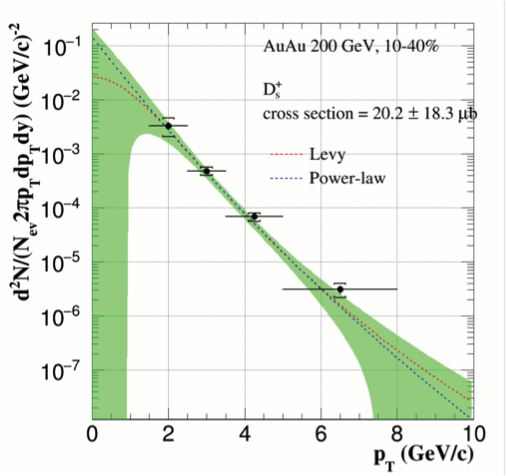
\includegraphics[width=1.0\textwidth,angle=0]{figure/Run14_D0HFT/ccx_3.png}
\caption{$D_{s}^{+}$ with the 10--40\% spectrum in Au + Au collisions fitted with the levy function and power low function used for the cross section calculation, then take the difference between two functions as the systematic uncertainties. \label{ccx_3}}
\end{minipage}
\hfill
\begin{minipage}[htbp]{0.47\linewidth}
\centering
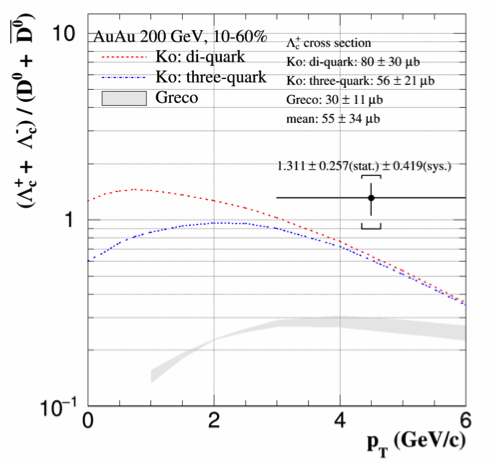
\includegraphics[width=1.0\textwidth,angle=0]{figure/Run14_D0HFT/ccx_4.png}
\caption{$\Lambda_{c}$ with the 10--60\% spectrum in Au + Au collisions fitted with the levy function and power low function used for the cross section calculation, then take the difference between two functions as the systematic uncertainties. \label{ccx_4}}
\end{minipage}
\end{figure}

\begin{figure}
\centering
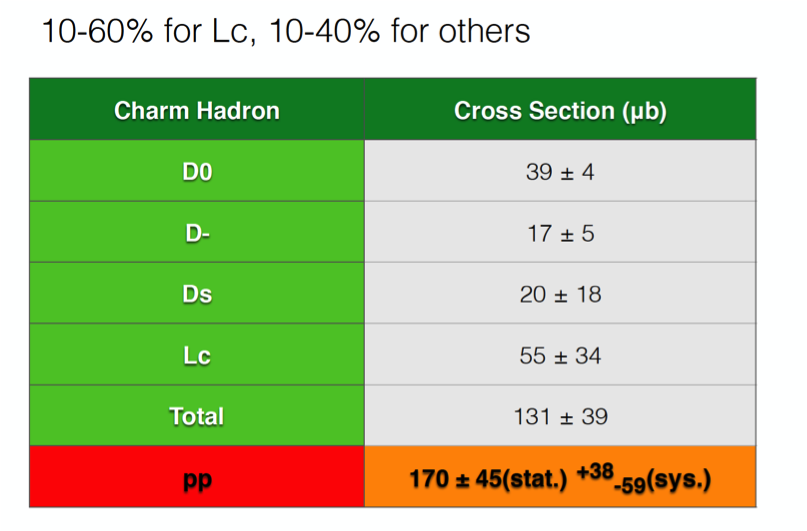
\includegraphics[width=0.68\textwidth]{figure/Run14_D0HFT/ccx_5.png}
\caption{table of the current ccbar cross section, also shown with pp.}
\label{ccx_5} 
\end{figure}

With the current ccbar cross section in Au + Au, also shown with in p + p, within the large uncertainties they are more or less comparable with the current precision.
